\documentclass[
	12pt,
	BCOR=5mm,
	DIV=12,
	footheight=30pt,
	headinclude=on,
	footinclude=off,
	parskip=half,
	bibliography=totoc,
	listof=entryprefix,
	toc=listof,
	numbers=noenddot,
	plainfootsepline]{scrreprt}
% !TEX root =  master.tex

%		LANGUAGE SETTINGS AND FONT ENCODING 
%
\usepackage[ngerman]{babel} 	% German language
\usepackage[utf8]{inputenc}
\usepackage[german=quotes]{csquotes} 	% correct quotes using \enquote{}
\usepackage[T1]{fontenc}
\usepackage{hyperref}

%\usepackage[english]{babel}   % For english language
%\usepackage{csquotes} 	% Richtiges Setzen der Anführungszeichen mit \enquote{}

% 		HYPERREF
%
%\usepackage[
%	hidelinks=true % keine roten Markierungen bei Links
%]{hyperref}

% Zwei eigene Befehle zum Setzen von Autor und Titel. Ausserdem werden die PDF-Informationen richtig gesetzt.
\newcommand{\TitelDerArbeit}[1]{\def\DerTitelDerArbeit{#1}\hypersetup{pdftitle={#1}}}
\newcommand{\AutorDerArbeit}[1]{\def\DerAutorDerArbeit{#1}\hypersetup{pdfauthor={#1}}}
\newcommand{\Firma}[1]{\def\DerNameDerFirma{#1}}
\newcommand{\Kurs}[1]{\def\DieKursbezeichnung{#1}}


% Correct superscripts 
\usepackage{fnpct}




%		CALCULATIONS
%
\usepackage{calc} % Used for extra space below footsepline



%		BIBLIOGRAPHY SETTINGS
%

% Uncomment the next three lines for author-year-style with footnotes (Chicago)
%\usepackage[backend=biber, autocite=footnote, style=alphabetic,citestyle=authoryear]{biblatex} 	
%Use Author-Year-Cites with footnotes
\usepackage[backend=biber, style=alphabetic, citestyle=alphabetic ]{biblatex} 	
%Use Author-Year-Cites with footnotes


\AdaptNoteOpt\footcite\multfootcite   %will add  separators if footcite is called multiple consecutive times 
\AdaptNoteOpt\autocite\multautocite % will add  separators if autocite is called multiple consecutive times

% Uncomment the next line for IEEE-style 
% \usepackage[backend=biber, autocite=inline, style=ieee]{biblatex} 	% Use IEEE-Style (e.g. [1])

% Uncomment the next line for alphabetic style 
% \usepackage[backend=biber, autocite=inline, style=alphabetic]{biblatex} 	% Use alphabetic style (e.g. [TGK12])

% Uncomment the next two lines vor Harvard-Style 
%\usepackage[backend=biber, style=apa]{biblatex} 	
%\DeclareLanguageMapping{german}{german-apa}


\DefineBibliographyStrings{ngerman}{  %Change u.a. to et al. (german only!)
	andothers = {{et\,al\adddot}},
}

%%% Uncomment the following lines to support hard URL breaks in bibliography 
%\apptocmd{\UrlBreaks}{\do\f\do\m}{}{}
%\setcounter{biburllcpenalty}{9000}% Kleinbuchstaben
%\setcounter{biburlucpenalty}{9000}% Großbuchstaben


\setlength{\bibparsep}{\parskip}		%add some space between biblatex entries in the bibliography
\addbibresource{quellen.bib}	%Add file bibliography.bib as biblatex resource


%		FOOTNOTES 
%
% Count footnotes over chapters
\usepackage{chngcntr}
\counterwithout{footnote}{chapter}
\usepackage{scrhack}
%	ACRONYMS
%%%
%%% WICHTIG: Installieren Sie das neueste Acronyms-Paket!!!
%%%
\makeatletter
\usepackage[printonlyused]{acronym}
\@ifpackagelater{acronym}{2015/03/20}
  {%
    \renewcommand*{\aclabelfont}[1]{\textbf{\textsf{\acsfont{#1}}}}
  }%
  {%
  }%
\makeatother

%		LISTINGS
\usepackage{listings}	%Format Listings properly
\renewcommand{\lstlistingname}{Quelltext} 
\renewcommand{\lstlistlistingname}{Quelltextverzeichnis}
\lstset{numbers=left,
	numberstyle=\tiny,
	captionpos=b,
	basicstyle=\ttfamily\small}


%		EXTRA PACKAGES
\usepackage{lipsum}    %Blindtext
\usepackage{graphicx} % use various graphics formats
\usepackage[german]{varioref} 	% nicer references \vref
\usepackage{caption}	%better Captions
\usepackage{booktabs} %nicer Tabs
\usepackage{array}
%\newcolumntype{P}[1]{>{\raggedright\arraybackslash}p{#1}}


%		ALGORITHMS
\usepackage{algorithm}
\usepackage{algpseudocode}
\renewcommand{\listalgorithmname}{Algorithmenverzeichnis }
\floatname{algorithm}{Algorithmus}


%		FONT SELECTION: Entweder Latin Modern oder Times / Helvetica
\usepackage{lmodern} %Latin modern font
%\usepackage{mathptmx}  %Helvetica / Times New Roman fonts (2 lines)
%\usepackage[scaled=.92]{helvet} %Helvetica / Times New Roman fonts (2 lines)

%		PAGE HEADER / FOOTER
%	    Warning: There are some redefinitions throughout the master.tex-file!  DON'T CHANGE THESE REDEFINITIONS!
\RequirePackage[automark,headsepline,footsepline]{scrlayer-scrpage}
\pagestyle{scrheadings}
\renewcommand*{\pnumfont}{\upshape\sffamily}
\renewcommand*{\headfont}{\upshape\sffamily}
\renewcommand*{\footfont}{\upshape\sffamily}
\renewcommand{\chaptermarkformat}{}
\RedeclareSectionCommand[beforeskip=0pt]{chapter}
\clearscrheadfoot

\ifoot[\rule{0pt}{\ht\strutbox+\dp\strutbox}DHBW Mannheim]{\rule{0pt}{\ht\strutbox+\dp\strutbox}DHBW Mannheim}
\ofoot[\rule{0pt}{\ht\strutbox+\dp\strutbox}\pagemark]{\rule{0pt}{\ht\strutbox+\dp\strutbox}\pagemark}

\ohead{\headmark}

% OTHER PACKAGES

\usepackage{textcomp}
\DeclareOldFontCommand{\sf}{\normalfont\sffamily}{\mathsf}
\usepackage{adjustbox}
\usepackage{epstopdf}
\usepackage{epsfig}
\usepackage{amssymb}
\usepackage{nameref}
\usepackage{theorem}
\usepackage{xcolor}
\usepackage{amsmath}
\usepackage{qtree}
\usepackage{multirow}
\usepackage{lmodern}
\usepackage{tabu}
\usepackage{xpicture}

\usepackage{hyperref}
\usepackage[all]{hypcap}
\hypersetup{
	colorlinks = true, % comment this to make xdvi work
	linkcolor  = blue,
	citecolor  = red,
        filecolor  = Gold,
        urlcolor   = [rgb]{0.5, 0.0, 0.5},
	pdfborder  = {0 0 0}
}

\definecolor{amethyst}{rgb}{0.2, 0.4, 0.6}
\definecolor{orange}{rgb}{1, 0.9, 0.0}
\definecolor{grey}{rgb}{0.5, 0.5, 0.5}

\newcommand{\blue}[1]{{\color{blue}#1}}
\newcommand{\green}[1]{{\color{green}#1}}
\newcommand{\red}[1]{{\color{red}#1}}
\newcommand{\grey}[1]{{\color{grey}#1}}
\newcommand{\el}{\!\in\!}

{\theorembodyfont{\sf}
\newtheorem{Definition}{Definition}
\newtheorem{Theorem}[Definition]{Theorem}
\newtheorem{Proposition}[Definition]{Proposition}
\newtheorem{Lemma}[Definition]{Lemma}
\newtheorem{Corollary}[Definition]{Corollary}
}


%------------------------------------------------------------------------------------
% Farben definieren
%------------------------------------------------------------------------------------
\definecolor{hellgelb}{rgb}{1,1,1} 
\definecolor{colKeys}{rgb}{0,0,1} 
\definecolor{colIdentifier}{rgb}{1,0,0} 
%\definecolor{colComments}{rgb}{0.66,0.66,0.66} 
\definecolor{colComments}{rgb}{0.5,0.5,0.5} 
\definecolor{colString}{rgb}{0,0.5,0} 
\usepackage[onehalfspacing]{setspace}
\definecolor{mxBlue}{RGB}{0,33,99}
%-------------------------------------------------------------------------------------

\usepackage{listings}

\lstset{
    float=hbp,
    basicstyle=\ttfamily\footnotesize,
    identifierstyle=\color{colIdentifier},
    keywordstyle=\color{mxBlue},
    stringstyle=\color{colString},
    commentstyle=\color{colComments},
    columns=flexible,
    tabsize=3,
    frame=single,
    extendedchars=false,
    showspaces=false,
    showstringspaces=false,
    numbers=right,
    numberstyle=\tiny,
    breaklines=false,
    backgroundcolor=\color{hellgelb},
    breakautoindent=false,
    captionpos=b
} 
%-----------------------------------------------------------------------------------
% C++ definieren
%-----------------------------------------------------------------------------------
\lstdefinelanguage{python}{
  keywords={new, true, false, def, return, null, catch, switch, for, if, in, while, do, else, case, break, cout, cerr, void, int , Json,length,Value, string, or , == },
  keywordstyle=\color{mxBlue}\bfseries,
  ndkeywords={class, boolean,ui,user_config_j ,system_config_j , this},
  ndkeywordstyle=\color{gray}\bfseries,
  identifierstyle=\color{black},
  sensitive=false,
  comment=[l]{\#},
  morecomment=[s]{"""}{"""},
  commentstyle=\color{colComments}\ttfamily,
  stringstyle=\color{red}\ttfamily,
  morestring=[b]',
  morestring=[b]"
}
%------------------------------------------------------------------------------------------------------------

% todo definieren ----------------------------------------------------
\usepackage[colorinlistoftodos,prependcaption,textsize=tiny]{todonotes}
\newcommand{\authorpatrick}{\todo[inline,linecolor=none,backgroundcolor=grey!25,bordercolor=black]{Patrick Müller}}
\newcommand{\authormax}{\todo[inline,linecolor=none,backgroundcolor=grey!25,bordercolor=black]{Max Zepnik}}
\newcommand{\unsure}[1]{\todo[linecolor=red,backgroundcolor=red!25,bordercolor=red]{#1}}
\newcommand{\change}[1]{\todo[linecolor=blue,backgroundcolor=blue!25,bordercolor=blue]{#1}}
\newcommand{\info}[1]{\todo[linecolor=green,backgroundcolor=green!25,bordercolor=green]{#1}}
\newcommand{\improvement}[1]{\todo[linecolor=lime,backgroundcolor=lime!25,bordercolor=lime]{#1}}
\newcommand{\thiswillnotshow}[1]{\todo[disable]{#1}}

%----Wörter formatieren-----------------------------------
\newcommand{\ot}{Othello}
\newcommand{\gtheorie}{Spieltheorie}
\newcommand{\board}{Board}
\newcommand{\state}{Spielzustand}
\newcommand{\states}{Spielzustands}
\newcommand{\gtree}{Spielbaum}
\newcommand{\gtrees}{Spielbaumes}
\newcommand{\code}[1]{\mxZitat{\texttt{#1}}} 
\newcommand{\mxZitat}[1]{\glqq{}#1\grqq{}} 
\newcommand{\abab}{Alpha\--Beta\--Ab\-schneiden}
\newcommand{\ababs}{Alpha\--Beta\--Ab\-schneidens}
\newcommand{\abp}{Alpha\--Beta\--Pru\-ning}
\newcommand{\mc}{Monte\--Carlo}
\vbadness=\maxdimen

\newcommand{\mxPicture}[5]{\XPicture{#1}{#2}{#3}{#4}{#5}}

\newcommand{\XPicture}[5]{\mxMinipage{\centering \XGraphic{#1}{#2} \captionof{figure}[#3]{#4} \vspace*{10pt} \label{#5} \vspace*{20pt} }}
\newcommand{\mxMinipage}[1]{\begin{minipage}{\textwidth} #1 \end{minipage}}
\newcommand{\XGraphic}[2]{\includegraphics[width=#1]{#2}}

\graphicspath{{./Bilder/}}

\title{Othello \\[0.3cm]
      --- Entwicklung einer KI für das Spiel ---}
\author{Patrick Müller, Max Zepnik}
\date{\today}

\newcommand{\so}[0]{\mathtt{S\textsubscript{0}}}


% später entfernen!! ---------------------------------------
\setlength {\marginparwidth }{2cm}
% ----------------------------------------------------------



\begin{document}
\TitelDerArbeit{Othello}
\UnterTitelDerArbeit{--- Entwicklung einer KI für das Spiel ---}
\AutorDerArbeit{Patrick Müller, Max Zepnik}
\Kurs{TINF16AIBI}

\begin{titlepage}
\begin{minipage}{\textwidth}
		\vspace{-2cm}
		\noindent \begin{center}
		
\includegraphics{Bilder/logo.jpg}
	\end{center}		 
\end{minipage}
\vspace{1em}
\sffamily
\begin{center}
	\textsf{\large{}Duale Hochschule Baden-Württemberg\\[1.5mm] Mannheim}\\[2em]
	\textsf{\textbf{\large{}Studienarbeit}}\\[3mm]
	\textsf{\textbf{\Large{}\DerTitelDerArbeit}} \\[0.3cm]
	\textsf{\textbf{\large{}\DerUnterTitelDerArbeit}} \\[1.5cm]
	\textsf{\textbf{\large{}Studiengang Angewandte Informatik}}%\\[3mm] \textsf{Studienrichtung Software Engineering}}
	
	%\vspace{3em}
	%\textsf{\Large{Sperrvermerk}}
\vfill

\begin{minipage}{\textwidth}

\begin{tabbing}
	Wissenschaftlicher Betreuer: \hspace{0.85cm}\=\kill
	Verfasser/in: \> \DerAutorDerArbeit \\[1.5mm]
	Matrikelnummer: \> 3409967, 9570942 \\[1.5mm]
	Kurs: \> \DieKursbezeichnung \\[1.5mm]
	Wissenschaftlicher Betreuer: \> Prof. Dr. Karl Stroetmann  \\
	Bearbeitungszeitraum: \> 17.09.2018 -- 29.04.2019
\end{tabbing}
\end{minipage}

\end{center}

\end{titlepage}
\pagenumbering{roman} % Römische Seitennummerierung
\addcontentsline{toc}{chapter}{Abstract}
\chapter*{Abstract}
\addcontentsline{toc}{section}{Deutsch}
\mxZitat{\ot} ist eine Variante des Spiels \mxZitat{Reversi}. Als klassisches Denkspiel wird es von zwei Spielern gegeneinander gespielt. Damit bietet es sich zur Umsetzung zu einem Spiel gegen den Computer an.
\\Ziel dieser Arbeit ist die Entwicklung von computergesteuerten Agenten, die einem menschlichen Spieler als Gegner zur Verfügung stehen.
\\Dabei wurden mehrere Agenten auf Grundlage der Strategien des \abab s (engl. \mxZitat{\abp}) sowie des \mc\ Algorithmus entwickelt. Zur Bewertung einzelner Spielzustände werden, sofern gemäß der Strategie erforderlich, Heuristiken herangezogen.
\\Als eine Heuristik wurde unter anderem die durchschnittliche Gewinnwahrscheinlichkeit als Ergebnis einer einzelnen Spielentscheidung herangezogen. Bei der Umsetzung dieses Ansatzes werden Symmetrieeigenschaften des Spielfeldes ausgenutzt.
\\Die beschriebenen Agenten werden in der Programmiersprache \mxZitat{Python} implementiert.
\\Zur Evaluierung werden die Ergebnisse der einzelnen Agenten im Spiel gegen einen zufällig agierenden Agenten, sowie untereinander betrachtet. Unter Verwendung der gesetzten Parameter kann dabei nur der auf dem \mc\ Algorithmus basierende Agent überzeugen.
\\Die auf der Betrachtung der durchschnittlichen Gewinnwahrscheinlichkeit als Ergebnis einer einzelnen Spielentscheidung basierende Heuristik kann im Vergleich mit anderen Heuristiken nicht überzeugen.

\begin{center}
***
\end{center}
\chapter*{Abstract}
\addcontentsline{toc}{section}{Englisch}

\mxZitat{\ot} is a variant of the game \mxZitat{Reversi}. As a classical game of thought it is played by two players against each other. By that, the game is well suited to be converted into a computer vs. human player game.
\\Therefore, the main goal of this paper is to develop computer-controlled agents available to act as opponents to human players.
\\In doing so, multiple agents were developed based on the strategies of \abp and the \mc\ Algorithms. If required by the strategy heuristics were used to evaluate individual game states.
\\Besides other heuristics one is based on the average probability of winning a game as a result to a specific decision during the game. The implementation of this approach relies upon symmetric properties of the playing field.
\\The agents described are implemented in the programming language \mxZitat{Python}.
\\For evaluation, the results of the agents against an agent performing random moves are considered as well as the results of the agents playing against each other. Using the parameters set for the evaluation, the agent based on the \mc\ algorithm is able to win the comparison.
\\The heuristic based on the average probability of winning a game as a result to a specific decision during the game is outperformed by other heuristics.
% !TEX root =  master.tex

%\clearpage
\chapter*{Ehrenwörtliche Erklärung}

% Wird die folgende Zeile auskommentiert, erscheint die ehrenwörtliche
% Erklärung im Inhaltsverzeichnis.

% \addcontentsline{toc}{chapter}{Ehrenwörtliche Erklärung}
Wir versichern hiermit, dass wir die vorliegende Arbeit  mit dem Thema:
\begin{center}
	\textsf{\textbf{\Large{}\DerTitelDerArbeit}} \\[0.3cm]
	\textsf{\textbf{\large{}\DerUnterTitelDerArbeit}} \\[1.5cm]
\end{center}
selbstständig verfasst und keine anderen als die angegebenen Quellen und Hilfsmittel benutzt haben.
\\Wir versichern zudem,
dass die eingereichte elektronische Fassung mit der gedruckten Fassung übereinstimmt.

\vspace{3cm}
Mannheim, \today
\\Ort, Datum \hfill Patrick Müller \hfill Max Zepnik

\normalfont

\tableofcontents
\addcontentsline{toc}{chapter}{Inhaltsverzeichnis}
\newpage

%	Abbildungsverzeichnis
\listoffigures

%	Tabellenverzeichnis
\listoftables

%	Listingsverzeichnis
\lstlistoflistings
\newpage

\pagenumbering{arabic}
\setcounter{page}{1}
\chapter{Einleitung}

%Umfeld - Othellos Gechichte
\mxZitat{\ot} ist eine Variante des, laut der Wikipedia, aus dem 19. Jahrhundert stammenden Spiels \mxZitat{Reversi} \cite{Wiki:EN:Reversi}. Als klassisches Denkspiel wird es von zwei Spielern gegeneinander gespielt. Die Beschreibung \mxZitat{Othello: A Minute to Learn, A Lifetime to Master} \cite{Rose} spiegelt dabei zwei wesentliche Aspekte wieder die es auszeichnen:
\\Die Anzahl der einfach gehaltenen Regeln hält sich in Grenzen und dennoch stellt es eine gewisse Herausforderung dar. Damit wird es zu einem einfach erlernbaren und kurzweiligen Spielerlebnis, dass es dem Spieler gestattet sich mit mehr und mehr Kenntnissen und Übungen stetig zu verbessern.
\\Damit bietet sich das Spiel zur Umsetzung zu einem Spiel gegen den Computer an.
%Ziel der Arbeit
\paragraph{Das Ziel dieser Arbeit} besteht darin eine Anwendung zu erstellen, die es einem menschlichen Spieler gestattet gegen Computergegner \mxZitat{\ot} zu spielen. Ein Anforderung an den Computeragenten besteht darin, dass er dem menschlichen Gegenspieler eine gewisse Schwierigkeit gegenüberstellt.
\\Als Grundvoraussetzung für einen dieser Anforderung entsprechenden Computeragenten wird dabei die Tatsache betrachtet, dass der Agent zumindest besser spielt als jener Agent der zufällig Züge durchführt.
%Betrachtungsgrenzen
\paragraph{Betrachtungsgrenzen}
Zur Beurteilung der Schwierigkeit, die ein Computergegner für einen menschlichen Spieler darstellt, bietet sich eine Gegenüberstellung der gewonnen Spiele im gemeinsamen Spiel an. Leider steht im Rahmen der Arbeit jedoch kein \ot\ Spieler zur Verfügung, der den Computeragenten auf einem gleichbleibend hohen Niveau testen könnte. Entsprechend fokussiert sich diese Arbeit auf den Vergleich des Computer Agenten mit einem zufällig spielenden Agenten bzw. den Vergleich verschiedener Algorithmen bzw. Spielstrategien untereinander.
%Aufbau der Arbeit
\newpage
\paragraph{Aufbau der Arbeit}
Die Arbeit ist dabei wie folgt aufgebaut:
\begin{enumerate}
\item Im Kapitel \ref{othello-chapter} werden die grundlegenden Begrifflichkeiten des Spiels sowie die Spielregeln eingeführt.
\item Danach werden im Kapitel \ref{basics} die zwei im weiteren Verlauf der Arbeit verwendeten Algorithmen mit ihren jeweiligen Variationen hergeleitet und erläutert.
\item Im Anschluss daran wird im Kapitel \ref{implementation} die im Rahmen der Arbeit entwickelte Implementierung der Spielmechanik sowie der Agenten vorgestellt und diskutiert.
\item Anhand der Implementierung werden die einzelnen Strategien dann evaluiert und bewertet bevor
\item im Kapitel \ref{Fazit} die Ergebnisse bewertet werden und ein Ausblick gegeben wird.
\end{enumerate}

\chapter{Othello}
\label{othello-chapter}
Von Othello gibt verschiedene Varianten. Eine Variante ist Reversi.
\info{weiter}
\\Othello wird auf einem 8x8 Spielbrett mit zwei Spielern gespielt. Es gibt je 64 Spielsteine, welche auf einer Seite schwarz, auf der anderen weiß sind. Der Startzustand besteht aus einem leeren Spielbrett, in welchem sich in der Mitte ein 2x2 Quadrat aus abwechselnd weißen und schwarzen Steinen befindet. Anschließend beginnt der Spieler mit den schwarzen Steinen.
%\mxPicture{5cm}{kategorie}{Koeffizientenmatrix }{Koeffizientenmatrix Q}{fig:quantisierung1}{}
Die Spielfelder werden in verschiedene Kategorien eingeteilt (siehe Abbildung
 \info{Abbildung}):
\begin{itemize}
\item Randfelder: äußere Felder
\item C-Felder: Felder, welche ein Feld horizontal oder vertikal von den Ecken entfernt sind
\item X-Felder: Felder, welche ein Feld diagonal von den Ecken entfernt sind
\item Zentrum: innerste Felder von C3 bis F6
\item Zentralfelder: Felder D4 bis E5
\item Frontsteine: die äußersten Steine auf dem Spielbrett um das Zentrum.
Viele dieser Tipps können auch im späteren Spielverlauf verwendet werden.
\end{itemize}
Diese Kategorien sind für die spätere Strategie wichtig.
\section{Spielregeln}
Othello besitzt einfache Spielregeln, welche im Spielverlauf aber auch taktisches oder strategisches Geschick erfordern. Jeder Spieler legt abwechselnd einen Stein auf das Spielbrett. Dabei sind folgende Spielregeln zu beachten:
\begin{itemize}
\item Ein Stein darf nur in ein leeres Feld gelegt werden.
\item Auf mindestens einer Seite des Steines (vertikal, horizontal oder diagonal) muss ein gegnerischer Stein durch diesen Stein umschlossen werden. Dies bedeutet, dass nach dem angrenzenden gegnerischen Stein beliebig viele generische Steine folgen und durch einen eigenen Stein abgeschlossen werden. Es dürfen sich keine leere Felder dazwischen befinden.
\item Die umschlossenen generischen Steine werden umgedreht, sodass alle Steine die eigene Farbe besitzen.
\item Ist für beide Spieler kein Zug mehr möglich, ist das Spiel beendet. Der Spieler mit den meisten Steinen seiner Farbe gewinnt das Spiel.
\end{itemize}
\improvement{spieler aussetzen }
\section{Spielverlauf}
Das Spiel wird in drei Abschnitte eingeteilt \cite{Ortiz.}:
\begin{itemize}
\item Eröffnungsphase
\item Mittelspiel
\item Endspiel
\end{itemize}
Diese Abschnitte sind jeweils 20 Spielzüge lang.
Im Eröffnungs- und Endspiel stehen zum Mittelspiel wenige Zugmöglichkeiten zur Verfügung, da entweder nur wenige Steine auf dem Spielbrett existieren oder das Spielbrett fast gefüllt ist und nur noch einzelne Lücken übrig sind. Im Mittelspiel existieren sehr viele Möglichkeiten, da sich schon mindestens 20 Steine auf dem Spielbrett befinden und diese sehr gute Anlegemöglichkeiten bieten. 
\section{Spielstrategien}
Wie in anderen Spielen gibt es auch in Othello verschiedene Strategien. Dabei kann beispielsweise offensiv gespielt werden, indem versucht wird möglichst viele Steine in einem Zug zu drehen. Es gibt auch defensive \mxZitat{stille} Züge. Ein \mxZitat{stiller} Zug dreht keinen Frontstein um und dreht möglichst nur wenige innere Steine um (vgl. \cite{Ortiz.}).
\\ Generell ist eine häufig genutzte Strategie die eigene Mobilität zu erhöhen und die Mobilität des Gegners zu verringern. Mit dem Begriff Mobilität sind die möglichen Zugmöglichkeiten gemeint. Durch das Einschränken der gegnerischen Mobilität hat dieser weniger Zugmöglichkeiten und muss so ggf. strategisch schlechtere Züge durchführen.
\\Die Position der Steine auf dem Spielbrett sollte ebenfalls nicht vernachlässigt werden.
beispielsweise sollen Züge auf X-Felder vermieden werden, da der Gegner dadurch Zugang zu den Ecken bekommt. Dadurch können ggf. die beiden Ränder und die Diagonale gedreht werden und in den Besitz des Gegners gelangen.
\\In der Eröffnungsphase sollten die Randfelder ebenfalls vermieden werden, da diese in dieser frühen Phase des Spiels noch gedreht werden können und der taktische Vorteil in einen strategischen Nachteil umgewandelt wird.
\section{Eröffnungszüge}
\label{othello-eroff}
In der nachfolgenden Tabelle \ref{tab:eroeffnungen} sind verschiedene Spieleröffnungen und deren Häufigkeit in Spielen aufgelistet. Spielzüge werden in Othello durch eine Angabe der Position, auf welche der Stein gesetzt wird, dargestellt. Ein vollständiges Spiel lässt sich deshalb in einer Reihe von maximal 60 Positionen darstellen.

\begin{table}[h]
  \centering
  \begin{tabular}{| c | c | c |}
    \hline
     Name & Häufigkeit & Spielzüge \\ \hline
     Tiger  &   47\%   & F5 D6 C3 D3 C4 \\ \hline
     Rose &   13\%   & F5 D6 C5 F4 E3 C6 D3 F6 E6 D7 \\ \hline
     Buffalo &  8\%    & F5 F6 E6 F4 C3 \\ \hline
     Heath  &  6\%    &  F5 F6 E6 F4 G5 \\ \hline
     Inoue &   5\%   &  F5 D6 C5 F4 E3 C6 E6\\ \hline
     Shaman &   3\%   & F5 D6 C5 F4 E3 C6 F3 \\ \hline
  \end{tabular}
  \caption{Liste von Othelloeröffnungen \cite{Ortiz.}}
  \label{tab:eroeffnungen}
\end{table}
\cite{Ortiz.} gibt folgende weitere Tipps für Eröffnungen:
\begin{itemize}
\item Versuche weniger Steinchen zu haben als dein Gegner.
\item Versuche das Zentrum zu besetzen.
\item Vermeide zu viele Frontsteine umzudrehen.
\item Versuche deine Steinchen in einem Haufen zu sammeln statt einige verstreute isolierte Steinchen zu haben.
\item Vermeide vor dem Mittelspiel auf die Kantenfelder zu setzen.
\end{itemize}
\unsure{Zitatweise ok?}

\chapter{Grundlagen}
\section{Spieltheorie}
\info{Einleitung fehlt}
\begin{Definition}[Spiel (Game)]
Ein \blue{Game} besteht aus einem Tupel der Form \\[0.2cm]
  \hspace*{1.3cm}
  $\mathcal{G} = \langle S\textsubscript{0},\mathtt{player}, \mathtt{actions}, \mathtt{result}, \mathtt{terminalTest}, \mathtt{utility} \rangle$
\\\so\ beschreibt den Startzustand des Spiels.
\\\textsc{player} ist auf der Menge der Spieler definiert und gibt den aktuellen Spieler zurück.
\\\textsc{actions} gibt die validen Folgezustände eines gegeben Zustands zurück.
\\\textsc{result} definiert das Resultat einer durchgeführten Aktion a und in einem Zustand s.
\\\textsc{terminalTest} prüft ob ein Zustand s ein Terminalzustand, also Endzustand, darstellt.
\\\textsc{utility} gibt einen Zahlenwert aus den Eingabenwerten s ( Terminalzustand) und p (Spieler) zurück. \\Positive Werte stellen einen Gewinn, negative Werte einen Verlust dar.
\info{quelle S.162}
\info{Definition States davor}
\end{Definition}
Eine spezielle Art von Spielen sind \blue{Nullsummenspiele}.
\begin{Definition}[Nullsummenspiele]
In einem \blue{Nullsummenspiel} ist die Summe der utility Funktion eines Zustands über alle Spieler 0. Dies bedeutet, dass wenn ein Spieler gewinnt mindestens ein Gegenspieler verliert.
\end{Definition}
Durch den Startzustand \so\ und der Funktion \textsc{action} wird ein \blue{Spielbaum (Game tree)} aufgespannt.
\begin{Definition}[Spielbaum (Game Tree)]
Ein \blue{Spielbaum} besteht aus einer einzigen Wurzel, welche einen bestimmten Zustand (meistens \so) darstellt. Die Kindknoten der Wurzel stellen die durch \textsc{actions} erzeugten Zustände dar. Die Kanten zwischen der Wurzel und den Kindknoten stellen jeweils die durchgeführte Aktion dar, die ausgeführt wurde um vom State s zum Kindknoten zu gelangen.
\end{Definition}
\begin{Definition}[Suchbaum (Search Tree)]
Ein \blue{Suchbaum} ist ein Teil des Spielbaums.
\end{Definition}
\cite{Russell.2016}
\info{Überleitung einfügen}
\section{Spielstrategien}
Es gibt verschiedene Spielstrategien. Im Folgenden werden diese kurz erläutert und anschließend verglichen.
\subsection{Min-Max}
\info{Patrick}
Der erste hier erläuterte Strategie ist der Min-Max Algorithmus. Dieser ist folgendermaßen definiert:
\\\Tree [.A [.B [.C eins ] [.D zwei ] ].B [.E {3 und 4} ] ].A
\subsection{Alpha-Beta Pruning}
\info{Max}
Der Min-Max Algorithmus berechnet nach dem Prinzip "depth-first" stets den kompletten Gametree. Bei der Betrachtung des Entscheidungsverhaltens des Algorithmus fällt jedoch schnell auf, dass ein nicht unerheblicher Teil aller möglichen Züge gar nicht erst in betracht gezogen wird. Dies geschieht aufgrund der Tatsache, dass diese Züge in einem schlechteren Ergebnis resultieren würden als die letzendlich ausgewählten.\newline
Dem \abp\ Algorithmus liegt der Gedanke zugrunde, dass die Zustände, die in einem realen Spiel nie auftreten würden auch nicht berechnet werden müssen. Damit steht die dafür regulär erforderliche Rechenzeit und der entsprechende Speicher dafür zur Verfügung andere, vielversprechendere Zweige zu verfolgen.
\subsubsection{Umsetzung}
Um die Umsetzung zu verdeutlcihen betrachten wir den folgenden, einfachen, Gametree. Unterhalb des Knotennamens wird jeweils das Ergebnis der MinMax-Funktion des Min-Max Algorithmus dargestellt.
\begin{figure}[h]
\caption[]{Beispielhafter Gametree}
\Tree [.{A\\a} [.{B\\5} [.{E\\5} ].{E\\5} [.{F\\13} ].{F\\13} [.{G\\8} ].{G\\8} ].{B\\5} [.{C\\6} [.{H\\h} ].{H\\h} [.{I\\i} ].{I\\i} [.{J\\j} ].{J\\j} ].{C\\c} [.{D\\d} [.{K\\k} ].{K\\k} [.{L\\l} ].{L\\l} [.{M\\m} ].{M\\m} ].{D\\d} ].{A\\a}
\end{figure}
\subsubsection{Ordnung der Züge}


\subsection{imperfect real time-time decisions}
\subsubsection{Evaluation functions}
\info{max}
\subsubsection{Cutting off search}
\info{max}
\subsubsection{Forward pruning}
\info{patrick}
\subsubsection{Search versus lookup}
\info{patrick}
\chapter{Implementierung der \ac{KI}}
\label{implementation}
In den folgenden Unterkapiteln werden verschiedene Spielalgorithmen vorgestellt und implementiert. Anschließend werden diese verbessert und auch unter Berücksichtigung des Laufzeitverhaltens analysiert.
\\Zunächst wird aber die grundsätzliche Programmstruktur erläutert und das Spielgerüst implementiert, damit unterschiedliche Spieler es ausführen können.
\section{Grundlegende Spiel-Elemente}
Die Python Implementierung befindet sich im Verzeichnis \mxZitat{python} des zu diesem Projekt gehörenden Git Repository. Um das Spiel zur Ausführung zu bringen werden die Pakete \mxZitat{numpy} sowie \mxZitat{pandas} benötigt. Sind diese Abhängigkeiten vorhanden, kann das Spiel durch das Ausführen des Kommandos \code{python3 main-game.py} gestartet werden. Es wird eine Pythonversion von 3.6.8 oder aktueller benötigt.
\\Die einzelnen Komponenten wurden unter thematischen Gesichtspunkten in verschiedenen Dateien organisiert. Nachfolgend wird auf die einzelnen Dateien und deren Funktion kurz eingegangen.
\subsection{Der Spielablauf}
In \mxZitat{main-game.py} wird das Rahmenprogramm gestartet. In diesem werden zunächst die Spieler festgelegt. Anschließend wird ein Spiel erstellt, initialisiert und das Spielbrett ausgegeben (siehe Listing \ref{lst:lst-main-game} Z. 2-4). Die Methode \code{game\_is\_over} gibt bei Spielende \code{True}, ansonsten \code{False} zurück. In der Schleife von Zeile 5 bis Zeile 12 wird der Agent des aktuellen Spielers ermittelt und der Übersicht halber ausgegeben (Z. 6f.). Für ihn wird dann die Funktion \code{get\_move} aufgerufen. Diese gibt den nach der Strategie des jeweiligen Agenten besten Spielzug zurück. Je nach Spielagent werden unterschiedliche Algorithmen zur Ermittlung dieses Zuges verwendet. Dieser Zug wird gespielt und auf das Spielbrett angewendet (Z. 10). Abschließend wird das aktualisierte Spielbrett und der zuletzt durchgeführte Zug ausgegeben (Z. 11f). Die Schleife wird bis zum Spielende wiederholt. Danach werden der Gewinner und die gesamte Spieldauer ermittelt und ausgegeben (Z. 13-16). 
\begin{lstlisting}[basicstyle=\footnotesize, caption = {Spielablauf in \mxZitat{main-game.py}}, language = python, captionpos = t , numbers=left, label={lst:lst-main-game}]
    players = {PLAYER_ONE: player_one, PLAYER_TWO: player_two}
    game = Othello()
    game.init_game()
    game.print_board()
    while not game.game_is_over():
        current_player = game.get_current_player()
        print(f"{PRINT_SYMBOLS[current_player]}'s turn:")
        player_object = players[current_player]
        move = player_object.get_move(game)
        game.play_position(move)
        game.print_board()
        print(f"Played position: ({COLUMN_NAMES[move[1]]}{move[0] + 1})")
    duration = time.time() - start
    print("Game is over")
    print(f"Total duration: {duration} seconds")
    print(f"Winner is {PRINT_SYMBOLS[game.get_winner()]}")
\end{lstlisting}
\subsection{Die Klasse \mxZitat{Othello}}
\label{ot1}
Die Klasse \mxZitat{Othello} modelliert einen Spielzustand und enthält die grundlegende Spiellogik wie bspw. die Berechnung erlaubter Züge. Nachfolgend wird auf die Art der Speicherung eines Spielzustandes und auf die wichtigsten Funktionen dieser Klasse eingegangen.
\paragraph{Klassenvariablen}
In Listing \ref{lst:class-vars-othello} sind alle Klassenvariablen, sowie deren Initialisierungswerte angegeben.
\begin{enumerate}
\item \code{\_board}: Bei \code{\_board} handelt es sich um ein Array des Paketes \code{numpy}, zur Modellierung der zweidimensionalen Struktur des Spielbretts. Initialisiert wird das Spielbrett in seinem Leerzustand. Daher wird zu Beginn jedes Feld auf den Wert der in \code{constants.py} definierten Integer-Konstante \code{EMPTY\_CELL} zur Repräsentation des leeren Feldes gesetzt.
\item \code{\_current\_player}: Speichert den Spieler, der im modellierten Spielzustand an der Reihe ist. Zur Repräsentation der Spieler werden die ebenfalls in \\\code{constants.py} definierten Integer-Konstanten \code{PLAYER\_ONE} und \\\code{PLAYER\_TWO} verwendet.
\item \code{\_last\_turn\_passed} wird verwendet, um zu speichern ob der vorherige Spieler passen musste. Dadurch kann das Spiel, sobald zwei Spieler unmittelbar nacheinander passen müssen, beendet werden.
\item \code{\_game\_is\_over} wird auf \code{True} gesetzt sobald das Spiel beendet ist.
\item \code{\_fringe}: In \code{\_fringe} werden alle Felder des Spielfeldes gespeichert die in eine Richtung unmittelbar neben einem bereits besetzten Feld liegen. Durch die Mitführung dieser Information muss zur Berechnung der erlaubten Züge nicht jedes Mal über das Spielfeld iteriert werden um zunächst die infrage kommenden Felder zu ermitteln.
\item \code{\_turning\_stones}: Ist ein Dictionary und enthält als Schlüssel alle erlaubten Züge und als Wert jeweils eine Liste jener Spielsteine, die durch das Ausführen des Zuges umgedreht werden. Da zur Ermittlung der erlaubten Züge diese Information bereits berechnet werden muss, wird sie in Form des Dictionary vorgehalten um diese an anderer Stelle nicht erneut berechnen zu müssen.
\item \code{\_taken\_moves}: Speichert alle ausgeführten Züge die erforderlich waren, um den modellierten Spielzustand zu erreichen, da einige Algorithmen diese Information benötigen.
\item \code{\_turn\_nr}: Speichert die Nummer des aktuellen Spielzuges, da die verwendete Strategie bei einigen Algorithmen davon abhängt, wie weit das Spiel schon fortgeschritten ist.
\item \code{\_number\_of\_occupied\_stones}: Speichert ein Dictionary welches für jeden Spieler die Anzahl der besetzten Felder mitführt. Dadurch muss dies zur Ermittlung des Gewinners nicht berechnet werden. Zur Repräsentation der Spieler werden ebenfalls die in \code{constants.py} definierten Integer-Konstanten \\\code{PLAYER\_ONE} und \code{PLAYER\_TWO} verwendet.
\end{enumerate}
\begin{lstlisting}[basicstyle=\footnotesize, caption = {Klassenvariablen der Klasse \mxZitat{Othello}}, language = python, captionpos = t , numbers=left, label={lst:class-vars-othello}]
    _board = np.full((8, 8), EMPTY_CELL, dtype='int8')
    _current_player = None 
    _last_turn_passed = False
    _game_is_over = False
    _fringe = set()
    _turning_stones = dict()    
    _taken_moves = []
    _turn_nr = 0
    _number_of_occupied_stones = {PLAYER_ONE: 0, PLAYER_TWO: 0}
\end{lstlisting}
\paragraph{Die Funktion \code{\_compute\_available\_moves}}
 ist in Listing \ref{lst:fct-compute-available-moves} angegeben und wird verwendet um die Inhalte des Dictionaries \code{\_turning\_stones} zu berechnen.
\\Da beiden Spielern in der Regel nicht die gleichen Züge zur Verfügung stehen, muss zunächst der vorherige Inhalt von \code{\_turning\_stones} gelöscht werden. Dies geschieht in Zeile 2, indem die Datenstruktur neu initialisiert wird.
\\In Zeile 3 wird eine lokale Referenz des zur Darstellung eines durch den aktuellen Spieler besetzen Feldes verwendeten Symbols erzeugt.
\\Mit der in Zeile 4 beginnenden Schleife wird über alle in Frage kommenden Züge in der Menge \code{\_fringe} iteriert, um zu ermitteln, ob dieser Zug erlaubt wäre.
\\Dazu wird zunächst eine lokale Menge initialisiert um die durch Spielen dieser Position gedrehten Steine zu speichern (Zeile 5).
\\Nun muss ausgehend von der derzeit betrachteten Position ermittelt werden, ob in irgendeine Richtung Spielsteine gedreht werden würden. Dies erfolgt durch die in Zeile 6 beginnende Schleife.
\\Dazu wird zunächst das nächste Feld in diese Richtung unter Verwendung einer Hilfsfunktion ermittelt (Zeile 7) und anschließend eine weitere temporäre Menge der in dieser Richtung gedrehten Steine initialisiert (Zeile 8).
\\Die entsprechende Richtung muss nun solange weiterverfolgt werden, wie ein weiterer Nachbar in diese Richtung vorhanden ist. Dies geschieht durch die in Zeile 9 beginnende Schleife.
\\Da in den nachfolgenden Schritten ermittelt werden muss, welcher Spieler das derzeit betrachtete Feld besetzt hat, werden die Indizes der derzeitigen Koordinaten ausgepackt (Zeile 10) und dann verwendet, um zu ermitteln welchen Wert das Feld derzeit hat (Zeile 11).
\\Nun gibt es drei mögliche Fälle:
\begin{enumerate}
\setcounter{enumi}{0}
\item Es befindet sich kein Stein auf dem derzeit betrachteten Feld. In diesem Fall wird die Abfrage in Zeile 12 positiv ausgewertet und diese Richtung muss nicht weiter verfolgt werden. Entsprechend wird die while-Schleife in Zeile 13 abgebrochen.
\item Das derzeit betrachtete Feld wird durch den anderen Spieler besetzt. In diesem Fall ist die Abfrage in Zeile 14 positiv. Da der Stein ggf. umgedreht werden würde, wird die aktuelle Position gespeichert (Zeile 15).
\item Das derzeit betrachtete Feld wird durch den Spieler selbst besetzt. In diesem Fall wird die Abfrage in Zeile 16 positiv ausgewertet. Nun würden alle Steine zwischen der Ausgangsposition und der derzeitigen gedreht. Daher wird die Menge der durch diesen Zug gedrehten Steine mit der der in diese Richtung befindlichen Steine vereinigt (Zeile 17) und die Schleife verlassen (Zeile 18).
\end{enumerate}
In Zeile 19 wird das nächste Feld in diese Richtung berechnet.
\\Gemäß der Regeln muss durch jeden Zug mindestens ein Stein gedreht werden. Aus diesem Grund wird nun ermittelt, ob dies bei diesem Zug gegeben wäre (Zeile 20). Ist dies der Fall, so werden die gedrehten Steine für diesen Zug in \code{\_stones\_to\_turn} gespeichert (Zeile 21).
\\Hat ein Spieler nun keine Möglichkeiten einen Zug durchzuführen, so sind in \\\code{\_stones\_to\_turn} keine Züge enthalten. Dieser Fall muss besonders behandelt werden. Tritt er ein, so wird die Abfrage in Zeile 22 positiv ausgewertet.
\\In diesem Fall muss nochmal unterschieden werden, ob der vorherige Spieler ebenfalls keinen Zug zur Auswahl hatte (Zeile 23).
\\Falls ja, so ist das Spiel zu Ende. Dies wird durch das Setzen von \code{\_game\_is\_over} gespeichert (Zeile 24).
\\Falls nein (Zeile 25), so wird gespeichert, dass der Spieler passen musste (Zeile 26) und der nächste Zug vorbereitet (Zeile 27).
\\Hat der Spieler hingegen eine Zugmöglichkeit (Zeile 28) so hat er aus Sicht des folgenden Zuges nicht passen müssen. Entsprechend wird \code{\_last\_turn\_passed} wieder auf \code{False} gesetzt. 
\newpage
\begin{lstlisting}[basicstyle=\footnotesize, caption = {Die Funktion \code{\_compute\_available\_moves}}, language = python, captionpos = t , numbers=left, label={lst:fct-compute-available-moves}]
    def _compute_available_moves(self):
        self._turning_stones = dict()
        player_value = self._current_player
        for current_position in self._fringe:
            position_turns = set()
            for direction in DIRECTIONS:
                next_step = Othello._next_step(current_position, direction)
                this_direction = set()
                while next_step is not None:
                    (current_row, current_column) = next_step
                    current_value = self._board[current_row][current_column]
                    if current_value == EMPTY_CELL:
                        break
                    elif current_value != player_value:
                        this_direction.add(next_step)
                    elif current_value == player_value:
                        position_turns |= this_direction
                        break
                    next_step = Othello._next_step(next_step, direction)
            if len(position_turns) > 0:
                self._turning_stones[current_position] = position_turns
        if len(self._turning_stones) == 0:
            if self._last_turn_passed:
                self._game_is_over = True
            else:
                self._last_turn_passed = True
                self._prepare_next_turn()
        else:
            self._last_turn_passed = False
\end{lstlisting}
\paragraph{Weitere Funktionen der Klasse \mxZitat{Othello}}
Die Klasse \mxZitat{Othello} enthält weitere Funktionen, auf welche hier jedoch nicht im Detail eingegangen werden soll. Dennoch sei hier jeweils kurz der Verwendungszweck der wichtigsten Funktionen genannt:
\begin{enumerate}
\item \code{set\_available\_moves} verändert \code{\_stones\_to\_turn} dahingehend, dass nur noch übergebene Positionen enthalten sind. Der Parameter kann damit zum Filtern der erlaubten Züge verwendet werden.
\item \code{play\_position} verändert den Spielzustand dahingehend, dass der übergebene Zug, sofern er erlaubt ist, ausgeführt wird, die entsprechenden Steine des Gegners gedreht und dessen Zug vorbereitet wird. Dabei wird auch die \code{\_fringe} entsprechend aktualisiert.
\item \code{get\_available\_moves}: Gibt die erlaubten Züge zur Verwendung in den \\Spielerimplementierungen zurück
\item \code{other\_player}: Gibt das Symbol des anderen Spielers zurück
\item \code{utility}: Gibt gemäß der Definition eines Spiels 0, 1 oder -1 zurück.
\item \code{get\_winner}: Ermittelt den Gewinner des Spiels und gibt ihn zurück.
\item \code{get\_statistics}: Gibt die Anzahl der Felder pro Spieler zurück.
\item \code{get\_current\_player}: Gibt den derzeitigen Spieler zurück.
\item \code{game\_is\_over}: Gibt zurück ob das Spiel bereits zu Ende ist.
\item \code{init\_game}: Bereitet den Start eines Spiels vor indem die initial besetzen Felder entsprechen gesetzt werden, der beginnende Spieler festgelegt und die  \code{\_fringe} vorbereitet, sowie \code{\_stones\_to\_turn} für den ersten Zug berechnet wird.
\item \code{deepcopy} und \code{init\_copy} Mittels dieser beiden Methoden ist es möglich eine sogenannte \mxZitat{tiefe} Kopie eines Spielzustandes anzufertigten. Die tiefe Kopie zeichnet sich dadurch aus, dass die im \code{Othello}-Objekt enthaltenen Objekte ebenfalls kopiert werden und nicht nur deren Referenzen. Dies ist erforderlich um den ursprünglichen Spielzustand bei der Durchführung eines simulierten Spiels, wie sie für diverse Spielalgorithmen erforderlich ist, nicht zu verändern. Die Verwendung der eingebauten Funktion \code{copy.deepcopy} kann hier nicht verwendet werden, da sie keine tiefe Kopie von \code{\_board} anfertigt.
\\Das Anfertigen von Kopien des \code{Othello}-Objektes während der Simulation von Spielen ist aus Performance Aspekten nicht zu vernachlässigen. Die Alternative bestünde darin Funktionen \code{push} und \code{pop} zu implementieren, die es erlauben mit einem \code{Othello}-Objekt simulierte Züge durchzuführen und rückgängig zu machen. Dieser Ansatz würde jedoch zum einen entweder das Kopieren des Ausgangszustandes oder das Mitführen von zahlreichen Zusatzinformationen erfordern um das Rückgängig machen eines Zuges ohne unvertretbar großen Rechenaufwand zu ermöglichen. Ob dies also einen tatsächlichen Performancevorteil bringt müsste daher seperat untersucht werden. Zum Anderen ist es, um mehrere Spiele parallel mittels mehrerer Prozesse ohne Schreib-Lese konflikte zu simulieren, erforderlich Kopien des \code{Othello}-Objektes anzulegen. Da ein Algorithmus jedoch genau dies erfordert wurde hier im Sinne der geringeren Code Komplexität auf die Implementierung der Methoden \code{pop} und \code{push} verzichtet.
\end{enumerate}
\subsection{Die übrigen Komponenten}
Neben den zuvor detailliert besprochenen, finden in der Implementierung noch die folgenden Komponenten Anwendung: 
\begin{enumerate}
\item Konstanten in der Datei \code{constants.py}. Durch die Verwendung von Konstanten bspw. zur Symbolisierung von welchem Spieler ein Feld besetzt ist, wird einerseits von konkreten Werten abstrahiert und dadurch sind diese, sofern erforderlich einfach austauschbar. Andererseits wird eine gewisse Konsistenz, bspw. für Mapping-Funktionen zur Ausgabe, über das ganze Programm hinweg erreicht.
\item Hilfsfunktionen in der Datei \code{util.py} werden dazu genutzt Werte vom Benutzer abzufragen.
\end{enumerate}
\newpage
\section{Heuristiken}
\label{heuristic}
Wie im Abschnitt \ref{Heuristiken} besprochen werden für einige Algorithmen Funktionen zur Approximation des Wertes eines Spielzustandes benötigt. Im Rahmen dieser Arbeit wurden die folgenden Heuristiken implementiert:
\begin{enumerate}
\item Nijssen Heuristik
\item Stored Monte-Carlo-Heuristik
\item Cowthello Heuristik
\end{enumerate}
In der Datei \code{heuristics.py} befinden sich die Implementierungen aller Heuristiken.

\subsection{Nijssen Heuristik}
\label{nissen2007H}
Die \mxZitat{Nijssen Heuristik} wurde aus \cite{nijssen_2007} übernommen. Ihr liegt die im Kapitel \ref{othello-chapter} erläuterte Idee zugrunde, die einzelnen Spielfelder in Kategorien einzuteilen und jeder Kategorie einen speziellen Wert zuzuweisen. Dieser Wert sei für jedes Feld $\mathtt{f} \in \mathtt{Moves}$ gegeben durch $w_{\mathtt{f}}$. 
\\Außerdem gebe es eine Funktion $\mathtt{occupiedBy}: \mathtt{Q} \times \mathtt{Moves} \times \mathtt{Players} \rightarrow \{-1, 0, 1 \}$ mit:
\\$\mathtt{occupiedBy}(\mathtt{s}, \mathtt{f}, \mathtt{p}) = \begin{cases}
1 & \, \text{wenn}\, \mathtt{f}\, \text{besetzt durch}\, \mathtt{p} \\
-1 & \, \text{wenn}\, \mathtt{f}\, \text{besetzt durch}\, \mathtt{other}(\mathtt{p}) \\
0 & \, \text{sonst}
\end{cases}$
\\Die Bewertung des Spielzustandes $\mathtt{s} \in \mathtt{Q}$ aus Sicht eines Spielers $\mathtt{p} \in \mathtt{Players}$ ergibt sich dann nach der folgenden Formel:  \vspace{0.25cm}\\ $\mathtt{heuristic}(\mathtt{s}, \mathtt{p}) = \sum\limits_{f \in \mathtt{Moves}}  \mathtt{occupiedBy}(\mathtt{s}, \mathtt{f}, \mathtt{p}) * w_{\mathtt{f}}$
\vspace{0.25cm}
\\Für die Gewichte $w_{\mathtt{f}}$ der im Kapitel \ref{othello-chapter} eingeführten Kategorien vergibt Nijssen die folgenden Werte:
\begin{itemize}
\item \code{Eck-Felder}: $+5$
\item \code{X-Felder}: $-2$
\item \code{C-Felder}: $-1$
\item \code{Zentral-Felder}: $+2$
\item \code{Andere-Felder}: $+1$
\end{itemize}
\subsection{Stored Monte-Carlo-Heuristik}
\label{impl:stored-mc}
Dieser Heuristik liegt die Idee zugrunde die in mehreren Spielen gesammelten Erkenntnisse zu den Gewinnchancen einzelner Züge zu speichern und in den darauffolgenden Spielen zur Beurteilung von Spielzuständen heranzuziehen.
\\Die von der \mxZitat{Stored Monte-Carlo-Heuristik} zu diesem Zweck verwendete Informationssammlung wird nachfolgend als Datenbank bezeichnet. In dieser Datenbank wird für jede Zugnummer, für jedes Feld des Spielfeldes Werte gespeichert, aus denen sich die Gewinnchance bei der Ausführung dieses Zuges zu diesem Spielzeitpunkt errechnen lassen. Um diese zu ermitteln wird eine große Anzahl zufälliger Spiele simuliert. Die gespeicherten Werte bestehen aus der Gesamtanzahl der simulierten Spiele, in welchen in diesem Zug, das jeweilige Feld besetzten wurde und, für jeden Spieler getrennt, die Häufigkeit, mit der der Spieler anschließend gewonnenen hat. Die genaue Funktion wird in den Unterabschnitten \nameref{para:db} und \nameref{para:train1} näher erklärt. Darauf aufbauend wird die Funktionsweise der Heuristik in dem Abschnitt \nameref{para:heuristic1} erläutert.
\paragraph{Datenbank}
\label{para:db}
Um die Anzahl der gespeicherten Werte zu verringern, werden die Symmetrieeigenschaften des Spielbretts ausgenutzt. 
So ist das Spielfeld ist symmetrisch zum Mittelpunkt aufgebaut. Dies bedeutet, dass Züge, welche symmetrisch zu anderen Zügen sind, als ein Zug angesehen werden können. Das Spielfeld wird daher in zehn Feldkategorien eingeteilt. In Abbildung \ref{fig:sym1} sind die symmetrischen Felder des Othello-Spielbrettes farblich hervorgehoben. Die unterschiedlichen Farben stellen die unterschiedlichen Feldkategorien dar. Diese sind von Null bis Acht durchnummeriert. Das Zentrum ist mit \mxZitat{X} markiert. Da das Zentrum bei Spielstart schon besetzt ist, wird diese Feldkategorie nicht in der Datenbank gespeichert. Mathematisch ist eine Feldkategorie eine disjunkte Teilmenge (Partition) aller Felder. Die restlichen neun Kategorien werden als Spalten in der Datenbank abgebildet, die in der Datei \code{database\_moves.csv} im CSV-Format realisiert ist.
\\\mxPicture{10cm}{symmetrie}{Symmetrie des Spielfeldes}{Symmetrie des Spielfeldes}{fig:sym1}{}
\\Die Datenbank besteht aus 60 Zeilen und neun Spalten. Die dreidimensionale Struktur wird zweidimensional dargestellt. Die neun Spalten stellen o.g. Feldkategorien (\mxZitat{0} bis \mxZitat{8} ohne \mxZitat{X}) dar. Die c-te Spalte in der n-ten Zeile stellt die Gewinnwahrscheinlichkeiten des Spieles dar, gegeben, dass im n-ten Spielzug ein Feld der Feldkategorie c gespielt wird. Die genaue Zuordnung der Spielkategorien sind in der Abbildung \ref{fig:sym1} dargestellt.
\\Jede Zelle in dieser Tabelle enthält nun ein Tripel der Form \\$( \mathtt{won\_games\_player\_1}, \mathtt{won\_games\_player\_2}, \mathtt{total\_played\_games})$. 
\\Die erste Komponente stellt die Anzahl der gewonnenen simulierten Spiele des ersten Spielers dar, die zweite Komponente speichert die Anzahl der Spiele, welche der zweite Spieler gewonnen hat und die dritte Komponente gibt die Gesamtanzahl der insgesamt simulierten Spiele dieser Spielkategorie an. Wie diese Werte ermittelt werden wird in Abschnitt \nameref{para:train1} erklärt.
\\Da Spiele unentschieden ausgehen können, gibt es zwischen den drei Komponenten den folgenden mathematischen Zusammenhang: 
\\$\mathtt{won\_games\_player\_1} + \mathtt{won\_games\_player\_2} \le \mathtt{total\_played\_games}$
\\In Abbildung \ref{fig:db1} ist der Initialzustand der Datenbank dargestellt (vgl. auch Abbildung \ref{fig:sym1} bzgl. der Feldkategorien). 
\\\mxPicture{13.5cm}{db2}{Ausschnitt des Initialzustandes der Datenbank}{Ausschnitt des Initialzustandes der Datenbank}{fig:db1}{}
Die Startwerte der Tupel sind jeweils \mxZitat{(0, 0, 0)}, da initial noch keine Spiele gespeichert sind.
\paragraph{Befüllen der Datenbank}
\label{para:train1}
Nachdem die Datenbank im vorherigen Abschnitt initialisiert erstellt wurde, wird diese nun mit Spieldaten aus zufällig gespielten Spielen befüllt. Dies wird in der Funktion \code{train\_db\_multi\_threaded(self, count)} durchgeführt, welche \code{count} Spiele spielt und mit deren Ergebnisse die Datenbank  aktualisiert. Die \code{count} Spiele werden gleichmäßig auf alle Prozessoren aufgeteilt und in der Funktion \code{\_play\_n\_random\_games(count)} durchgeführt. In dieser Funktion spielen zwei \mxZitat{Random}-Agenten gegeneinander. Die daraus gewonnenen Spielinformationen (Zugreihenfolge, Gewinner des Spiels) werden von der Funktion \code{update\_fields\_\\stats\_for\_single\_game} verarbeitet. 
\\In Listing \ref{lst:train1} ist das Spielen eines einzelnen zufälligen Spieles und den Aufruf der Funktion \code{update\_fields\_stats\_for\_single\_game} abgebildet. Das Listing ist eine Zusammenstellung von Auszügen der Funktionen \code{\_play\_n\_random\_games} und \code{train\_db\_multi\_threaded}. Zunächst wird ein Othello-Spiel initialisiert (Z. 1f.). Durch die Nutzung des im Kapitel \ref{agenten} näher erläuterten \mxZitat{Random}-Agenten wird ein komplettes Spiel durchgeführt (Z. 3f). Anschließend wird der Gewinner (Z. 5) und die Zugreihenfolge ermittelt (Z. 6). Die Funktion \code{update\_fields\_stats\_for\_""single\_game} verwendet diese beiden Parameter, um die Datenbank zu aktualisieren. Sie wird in Listing \ref{lst:train2} abgebildet.
\newpage
\begin{lstlisting}[basicstyle=\footnotesize, caption = {Befüllen der Datenbank 1}, language = python, captionpos = t , numbers=left, label={lst:train1}]
g = Othello()
g.init_game()
while not g.game_is_over():
	g.play_position(Random.get_move(g))
winner = g.get_winner()
moves = g.get_taken_mv()
self.update_fields_stats_for_single_game(moves, winner)
\end{lstlisting}
In der Funktion \code{update\_fields\_stats\_for\_single\_game} (Listing \ref{lst:train2} Z. 9-12) wird die Liste der Züge in einzelne Züge aufgeteilt (Z. 13), welche anschließend jeweils eine Spalte in einer Datenbankzeile aktualisieren. Dazu werden die Züge, beispielsweise \mxZitat{a1}, in Zeile 15 in eine Feldkategorie umgerechnet (im Beispiel \mxZitat{0}) und ebenfalls der Methode \code{update\_field\_stat} übergeben (Z. 17).
\\Diese Methode liest die Werte der durch Zugnummer und Feldkategorie festgelegten Zelle aus (Z. 2f.). Je nachdem, welcher Spieler dieses Spiel gewonnen hat, wird die Zahl der gewonnenen Spiele des ersten, zweiten oder keinem Spieler um eins erhöht (Z. 4-7). Abschließend wird die Zahl der insgesamt durchgeführten Spiele inkrementiert (Z. 10 dritte Komponente) und in die Datenbank zurückgeschrieben (Z. 9f.).
\\Die Datenbank wurde mit 140.000 Spielen trainiert, um statistische Abweichungen zu minimieren. Hierbei wirkt das Gesetz der großen Zahlen, das besagt, dass sich die Wahrscheinlichkeiten eines Ereignisses bei sehr vielen Wiederholungen dem Erwartungswert annähert.
\\Zur Auswertung der Datenbank wurde die Klasse \code{Analyse} in der Datei \\\code{analyse\_database.py} erstellt. Diese liest die Datenbank aus und liefert eine farbige Ansicht der Gewinnwahrscheinlichkeiten eines Spielers jeweils pro Zug auf dem Terminal. Neben dem dargestellten Spielbrett wird auch das Minimum, das Maximum, der Durchschnittswert und die Standardabweichung des dargestellten Spielbrettes berechnet. Zur Nutzung dieser Funktion wird das python-Paket \mxZitat{termcolor} benötigt.
\newpage
\begin{lstlisting}[basicstyle=\footnotesize, caption = {Befüllen der Datenbank 2}, language = python, captionpos = t , numbers=left, label={lst:train2}]
	    def update_field_stat(self, turn_nr, field_type, winner):
        (won_games_pl1, won_games_pl2, total_games_played) = \
        	self._db_data[turn_nr][field_type]
        if winner == PLAYER_ONE:
            won_games_pl1 += 1
        elif winner == PLAYER_TWO:
            won_games_pl2 += 1
        # store updated entry at same position in database
        self._db_data[turn_nr][field_type] = \
        	(won_games_pl1, won_games_pl2, total_games_played + 1)

    def update_fields_stats_for_single_game(self, moves, winner):
        for turn_nr in enumerate(moves):
            # translate move 1,0 to position 8
            position = POSITION_TO_DATABASE[moves[turn_nr]]
            # update array at position position
            self.update_field_stat(turn_nr, position, winner)
\end{lstlisting}

\paragraph{Heuristik}
\label{para:heuristic1}
Mithilfe der o.g. Datenbank wird  nun eine Heuristik zur Bewertung eines Spielzustandes implementiert.
\\Um nun zu erläutern wie die Ausführung eines einzelnen Zuges bewertet wird werden zunächst die folgenden Mengen bzw. Funktionen benötigt:
\\$\mathtt{Categories}: \{ 0,...,8\} $: Menge der definierten Feldkategorien
\\$\mathtt{category}: \mathtt{Moves} \rightarrow \mathtt{Categories}$: Gibt die Feldkategorie eines einzelnen Spielfeldes zurück.
\\$\mathtt{database}: \mathbb{N} \times \mathtt{Categories} \rightarrow < \mathbb{N} ,\mathbb{N} ,\mathbb{N}>$: Gibt ein Tripel bestehend aus Anzahl gewonnener Spiele des ersten, bzw. zweiten Spielers und Gesamtanzahl der Spiele zurück. Bietet damit eine Möglichkeit zum Zugriff auf die in der Datenbank gespeicherten Informationen.
\\$\mathtt{w}: < \mathbb{N} ,\mathbb{N} ,\mathbb{N}> \times\ \mathtt{Players} \rightarrow \mathbb{N}$ : Erwartet ein Tripel wie es von der Funktion \code{database} zurückgegeben wird und gibt daraus die Anzahl der Gewinne des übergebenen Spielers zurück.
\\$\mathtt{t}: < \mathbb{N} ,\mathbb{N} ,\mathbb{N}> \times\ \mathtt{Players} \rightarrow \mathbb{N}$ : Erwartet ein Tripel wie es von der Funktion \code{database} zurückgegeben wird und gibt daraus die Anzahl der insgesamt simulierten Spiele zurück.
\\$\mathtt{turn}: \mathtt{Q} \rightarrow \mathbb{N} $ : Gibt die Anzahl der durchgeführten Züge um einen Zustand zu erreichen an.
\\Damit kann nun die Definition der Bewertungsfunktion vorgenommen werden:
\\Für einen Spielzustand $\mathtt{s} \in \mathtt{Q}$ wird die Durchführung eines Zuges $\mathtt{m} \in \mathtt{actions}(s)$ wie folgt bewertet:
\\$\mathtt{stored\_mc\_heuristic}(\mathtt{s}, \mathtt{m}) = \frac{\mathtt{w}(\mathtt{database}(\mathtt{turn}(\mathtt{s}),\mathtt{category}(\mathtt{m})),\mathtt{player}(\mathtt{s}))}{\mathtt{t}(\mathtt{database}(\mathtt{turn}(\mathtt{s}),\mathtt{category}(\mathtt{m})),\mathtt{player}(\mathtt{s}))} $
\\Umgesetzt ist dies in der Methode \code{heuristic} die in Listing \ref{lst:heuristic2} abgebildet ist. Diese ermittelt die verfügbaren Zugmöglichkeiten und die aktuelle Zugnummer (Z. 2f). Für jede Zugmöglichkeit wird die Gewinnwahrscheinlichkeit für den übergebenen Spieler in eine Wörterbuch-Datenstruktur gespeichert (Z. 6f). Aus dieser Datenstruktur wird die höchste Wahrscheinlichkeit ermittelt und zurückgegeben (Z. 9f).
\begin{lstlisting}[basicstyle=\footnotesize, caption = {Stored Monte-Carlo-Heuristik Funktion}, language = python, captionpos = t , numbers=left, label={lst:heuristic2}]
def heuristic(current_player, game_state: Othello):
	moves = game_state.get_available_moves()
	turn_nr = game_state.get_turn_nr()
	move_probability = dict()

	for move in moves:
		move_probability[move] = database.db.get_likelihood(move, turn_nr, current_player)

	selected_move = max(move_probability.items(), key=operator.itemgetter(1))[0]
 	return move_probability[selected_move]
\end{lstlisting}

\subsection{Cowthello Heuristik}
Die \mxZitat{Cowthello Heuristik} wurde aus \cite{cow1} übernommen. Ihr liegt ebenfalls der in Kapitel \ref{othello-chapter} erläuterte Ansatz zugrunde, die einzelnen Spielfelder in Kategorien einzuteilen und jeder Kategorie einen speziellen Wert zuzuweisen. Die Heuristik unterscheidet sich von der \nameref{nissen2007H} nur in der genaueren Definition der Feldkategorien und unterschiedliche Gewichtungen dieser Felder.
Die Gewichte der einzelnen Felder sind in Abbildung dargestellt. Die Unterschiede zur \nameref{nissen2007H} bestehen in der detaillierteren Gewichtung beispielsweise der Zentralfelder (\mxZitat{1}, \mxZitat{5} oder \mxZitat{50}) im Gegensatz zu \mxZitat{2}. Die restliche Implementierung ist identisch zur \nameref{nissen2007H}.
\\\mxPicture{10cm}{cow1}{Gewichtung der einzelnen Spielfelder}{Gewichtung der einzelnen Spielfelder}{fig:cow1}{}
In der Abbildung \ref{fig:cow1} wird deutlich, dass die Werte strategisch zugewiesen wurden. Beispielsweise sind die \mxZitat{X}- und \mxZitat{C}-Felder mit \mxZitat{schlechten} Werten (\mxZitat{-50}, \mxZitat{-25}) belegt. Dies spiegelt auch die Spielstrategie wider, dass diese Felder für den aktuellen Spieler schlecht sind, da der Gegner dadurch leicht eine Ecke des Spielfeldes besetzen kann.
\section{Start Tabellen}
In dem Grundlagenkapitel \ref{lookup} wurden die Vor- und Nachteile von Suche vs. Nachschlagen beschrieben. In diesem Kapitel wird darauf aufbauend die Implementierung zur Verwendung von einer Eröffnungsbibliothek, in der zu Beginn des Spiels bewährte Züge nachgeschlagen werden können, erläutert. In dieser Arbeit wird ein solche Bibliothek synonym mit Spieltabellen und Startdatenbank bezeichnet, da diese als eine Arte Tabelle in einer Datenbank gespeichert werden.
\\Für viele Spiele, beispielsweise für Schach, existieren umfangreiche Eröffnungsbibliotheken, welche bewährte Eröffnungszüge speichern. Für Othello existieren zwar viele Sammlungen von durchgeführten Spielen, jedoch sind den Verfassern nur wenige Eröffnungsspiele bekannt. In der hier präsentierten Implementierung werden die 77 Eröffnungszüge von Robert Gatliff \cite{open1} verwendet. Beschrieben werden diese jeweils durch eine Zugreihenfolge, z.B. \code{c4, c3, d3, c5, b2}. 
\\Die zur Erreichung des aktuellen Spielzustandes gespielten Züge werden mit den gespeicherten Zugreihenfolgen verglichen. Wenn diese Reihenfolgen für eine oder mehrere gespeicherte Eröffnungen übereinstimmen, wird eine dieser Reihenfolgen ausgewählt und der nach dieser Reihenfolge nächste Zug gespielt. Die entsprechende Funktion \code{get\_available\_moves\_of\_start\_tables} ist in Listing \ref{lst:start2} abgebildet.
\begin{lstlisting}[basicstyle=\footnotesize, caption = {Methode zur Bestimmung verfügbarer Startzüge }, language = python, captionpos = t , numbers=left, label={lst:start2}]
def get_available_moves_of_start_tables(self, game: Othello):
	if len(self._start_tables) == 0:
		self._init_start_tables()
	turn_nr = game.get_turn_nr()
	available_moves = []
	taken_mv = game.get_taken_mvs_text()
	for game in self._start_tables:
		turn = 0
		for move in game:
			if turn < turn_nr:
				if taken_mv[turn] != move:
					break
			elif move != "i8" or move != "nan":  # invalid field
				available_moves.append(move)
				break
			turn += 1
	available_moves = list(dict.fromkeys(available_moves))
	if "nan" in available_moves:
		available_moves.remove("nan")
	return available_moves
\end{lstlisting}
Beim ersten Aufrufen der Starttabellen, wird die Datenbank initialisiert (Z. 2f). Ab Zeile sieben werden alle Zeilen der Datenbank mit der aktuellen Zugreihenfolge des Spiels verglichen (Z. 9ff). Wenn ein Zug in der bestehenden Zugreihenfolge abweichend von dem aktuellen Eintrag der Startdatenbank ist (Z. 11f), wird der weitere Vergleich mit diesem Eintrag abgebrochen und mit dem folgenden Eintrag fortgefahren.
\\Da das Spielbrett symmetrisch zum Mittelpunkt ist, wurden die von Robert Gatliff \cite{open1} übernommenen Eröffnungszüge entsprechend gespiegelt. Dadurch wurde die Datenbank auf 308 Züge erweitert. Diese ist in der Datei \code{start\_moves.csv} als CSV gespeichert.
\\Die Agenten (siehe dazu Kapitel \ref{agenten}) \mxZitat{\mc} und \mxZitat{\abp} verwenden in der Standardeinstellung diese Starttabellen. Wenn beide Agenten gegeneinander spielen, werden die ersten Spielzüge beider Spieler sehr stark beschleunigt. Die Agenten müssen keine Züge berechnen, sondern können, bei verfügbaren Eröffnungszügen, durch das Nachschlagen in der Datenbank und die Auswahl eines Spielzuges sehr viel Spielzeit einsparen. Erst wenn die Datenbank keine passende Zugreihenfolge mehr enthält, starten die Agenten die Berechnung des, nach der jeweiligen Strategie, besten Zuges. Ist sich ein Spieler dieser Tatsache bewusst, so kann er gezielt solche Zugfolgen spielen die eher ungewöhnlich und damit nicht in der Sammlung enthalten sind. In diesem Fall geht der durch die Sammlung möglicherweise erzielte Vorteil verloren.
\section{Agenten}
\label{agenten}
Beim Start einer Partie stehen dem Nutzer mehrere Agenten zur Auswahl die die Rolle eines Spielers übernehmen können. Die Implementierung zu diesen Agenten befindet sich in Unterverzeichnis \code{Agents}.
\\Die folgenden Agenten stehen dabei zur Auswahl:
\begin{enumerate}
\item \mxZitat{Human}
\item \mxZitat{Random Player}
\item \mxZitat{\mc}
\item \mxZitat{\abp}
\end{enumerate}
\subsection{Human Agent}
Der \mxZitat{Human Agent} bzw. menschliche Agent stellt eine Schnittstelle, die es einem menschlichen Spieler ermöglicht eine Spielentscheidung zu treffen, dar. Die Implementierung findet sich in der Datei \code{human.py}
\\Neben dem Spielfeld bekommt der Nutzer dabei eine Liste aller für Ihn möglichen Züge dargestellt. Durch die Eingabe eines Zuges wird dieser im Spielmodell ausgeführt und der nächste Agent wird aufgerufen. Da das Ziel dieser Arbeit darin besteht eine \ac{KI} zur Wahl der Züge zu entwickeln, soll an dieser Stelle nicht weiter auf diesen Agenten eingegangen werden.

\subsection{Random}
Die Implementierung des Agenten \mxZitat{Random} befindet sich in der Datei \code{random.py}. Dieser Agent ist die einfachste Form der im Rahmen dieser Arbeit eingesetzten Strategien einer \ac{KI}. Ihr liegt die Idee zugrunde, dass der Agent einen zufälligen Zug aus der Menge der erlaubten Züge auswählt.
\\In der mit der Arbeit entwickelten Implementierung ist dies derartig umgesetzt, dass der Agent die Liste der möglichen Züge aus dem Spielzustand abruft und einen zufälligen Index der Liste auswählt, um dann den dort angegebenen Zug zu spielen.

\subsection{\mc}
Hinter diesem Agenten steht das im Kapitel \ref{mc_algo} erläuterte Prinzip, der zufällig gespielten Spiele zur Ermittlung des Spielzuges mit der höchsten Gewinnwahrscheinlichkeit. Dabei werden ausgehend von einem derzeitigen Spielzustand $N$ Spiele simuliert in dem für beide Spieler der Agent \mxZitat{Random} verwendet wird. Dabei wird für den jeweils ersten simulierten Zug gespeichert wie oft dieser durchgeführt wurde und wie häufig dies in einer gewonnenen Simulation resultierte. In dem nicht simulierten Spiel wird dann jener Spielzug ausgeführt, bei dem der Quotient aus der Anzahl der nach dem Spielen dieses Zuges gewonnenen Spiele und der Anzahl der simulierten Spiele, die mit diesem Zug begonnen wurden, am größten ist.
\\Nachfolgend wird dieses Prinzip anhand des Quellcodes nochmals erläutert.
\\Die Spielerklasse \mxZitat{MonteCarlo} ist in der Datei \code{monteCarlo.py} zu finden.
\subsubsection{Parameter}
\label{mc_params}
Das genaue Verhalten des Agenten kann durch die folgenden Parameter beeinflusst werden: 
\begin{itemize}
\item \code{big\_n}: Die Anzahl $N$ der zufällig gespielten Spiele je Entscheidung
\item \code{use\_start\_libs}: Bool'scher Wert der angibt ob Startbibliotheken verwendet werden sollen
\item \code{preprocessor}: Der verwendete Vorverarbeiter bzw. Präprozessor. Dabei stehen die folgenden bereits im Kapitel \ref{mc_algo} besprochenen Varianten zur Auswahl:
\begin{itemize}
    \item Der feste Selektivität Präprozessor
    \item Der variable Selektivität Präprozessor
    \item Kein Präprozessor
\end{itemize}
\item \code{preprocessor\_parameter}: Parameter des verwendeten Präprozessors. Je nach Auswahl des Präprozessors steht dieser Parameter für:
\begin{itemize}
    \item Die Anzahl der Züge die durch den Präprozessor gelangen
    \item Die prozentuale Abweichung vom Mittelwert der Wertigkeiten der Züge
\end{itemize}
\item \code{heuristic}: Eine der in  Kapitel \ref{heuristic} beschriebenen. Wird im Präprozessor zur Bewertung von Spielzuständen herangezogen.
\item \code{use\_multiprocessing}: Bool'scher Wert, der angibt ob die $N$ simulierten Spiele unter Verwendung mehrerer Prozesse durchgeführt werden sollen. Bei Systemen mit mehr als einem Prozessor können damit durch Parallelisierung Geschwindigkeitsvorteile erreicht werden. 
\item \code{use\_weighted\_random}: Bool'scher Wert, der angibt ob die Züge mit einer höheren Gewinnwahrscheinlichkeit stärker in der Random Funktion gewichtet werden sollen.
\end{itemize}

\subsubsection{Die Präprozessoren}
Nachfolgend wird kurz auf die Implementierung der in Kapitel \ref{mc_algo} beschriebenen Präprozessoren eingegangen.
\paragraph{Der feste Selektivität Präprozessor}
Die in Listing \ref{lst:mc-prep-fixed} abgedruckte Funktion gibt die Implementierung des Präprozessors mit fester Selektivität an.
\\Die Funktion erhält einen Spielzustand \code{game\_state}, den Parameter \code{n\_s} der Anzahl $N_{s}$ der Züge, die den Präprozessor passieren und eine Heuristik \code{heuristic}, die zur Bewertung der Spielzüge herangezogen wird. In der sich über die Zeilen 3 bis 5 erstreckenden Anweisung wird eine nach der Bewertung des einzelnen Zuges gemäß der Heuristik sortierte Liste von Zügen erstellt. In Zeile 6 werden dann nur die ersten \code{n\_s} Züge im Spielzustand \code{game\_state} gesetzt.
\begin{lstlisting}[basicstyle=\footnotesize, caption = {Die Funktion \code{preprocess\_fixed\_slectivity}}, language = python, captionpos = t , numbers=left, label={lst:mc-prep-fixed}]
	@staticmethod	    
	def preprocess_fixed_selectivity(game_state: Othello, n_s, heuristic):
    heuristic_values = sorted(
        MonteCarlo.preprocess_get_heuristic_value(game_state, heuristic=heuristic).items(),
            key=operator.itemgetter(1))
    game_state.set_available_moves(heuristic_values[:n_s][0])
\end{lstlisting}
\paragraph{Der variable Selektivität Präprozessor}
In Listing \ref{lst:mc-prep-var} ist die Implementierung des Präprozessors mit variabler Selektivität angegeben.
\\Wie der Präprozessor mit fester Selektivität, erhält auch diese Funktion einen Spielzustand \code{game\_state} und eine Heuristik \code{heuristic}. Anders als bei dem oben beschriebenen Präprozessor wird hier jedoch ein Wert \code{p\_s} zur Beschreibung der maximalen prozentualen Abweichung $p_{s}$ vom Mittelwert der Wertigkeit der Züge übergeben.
\\Für die Berechnung wird zunächst der Wert der Heuristik für alle Spielzüge ermittelt (Zeile 3). Daraufhin wird in der Zeile 5 der durchschnittliche Wert berechnet und mit der Anweisung in den Zeilen 6 und 7 nur jene Züge im Spielzustand gesetzt, die einen Wert größer als $p_{s}$ multipliziert mit dem durchschnittlichen Wert haben.
\newpage
\begin{lstlisting}[basicstyle=\footnotesize, caption = {Die Funktion \code{preprocess\_variable\_slectivity}}, language = python, captionpos = t , numbers=left, label={lst:mc-prep-var}]
	@staticmethod
    def preprocess_variable_selectivity(game_state: Othello, p_s, heuristic):
        heuristic_value_dict = MonteCarlo.preprocess_get_heuristic_value(
        		game_state, heuristic=heuristic)
        heuristic_values = [v for _, v in heuristic_value_dict.items()]
        average_heuristic_value = sum(heuristic_values) / len(heuristic_values)
        game_state.set_available_moves(
            [m for m, v in heuristic_value_dict.items() if v >= p_s * average_heuristic_value])
\end{lstlisting}
\subsubsection{Die Funktion \code{get\_move}}
\label{mc-getmove}
Eine Funktion \code{get\_move} wird von allen Agenten bereitgestellt und in der \\\code{main-game.py} zur Auswahl eines Zuges gerufen. Beschrieben wird der Zug durch ein Paar, welches die Koordinaten auf dem Spielbrett darstellt.
\\Nachfolgend wird die in Listing \ref{lst:getmovemc} abgedruckte Funktion diskutiert:
\vspace{0.5cm}
\\Als Parameter erhält die Funktion den Spielzustand \code{game\state}, zu dem die Entscheidung über den nächsten Zug getroffen werden soll. In Zeile 2 wird nun überprüft, ob die Verwendung der Starttabellen aktiviert ist und zusätzlich in dem aktuellen Spiel weniger als 21 Züge gespielt wurden. Die zweite Komponente der \code{if}-Abfrage erfolgt, da die Startbibliothek maximal Strategien bis zum 20-ten Zug enthält.
\\Ist dies der Fall, so werden in Zeile 3 alle gemäß der Startbibliothek in Frage kommenden Züge ermittelt. Steht mindestens ein Zug zur Auswahl (Z. 4), so wird dieser gespielt (Z. 5). Nun werden die im vorherigen Zug ermittelten Wahrscheinlichkeiten gelöscht (Z. 6) und das Symbol, welches zur Repräsentation des eigenen Spielers verwendet wird zwischengespeichert (Z. 6).
\\Ist die Option zur Verwendung eines Präprozessors aktiviert, wird die Abfrage in Zeile 8 positiv ausgewertet. In diesem Fall wird der selektierte Präprozessor aufgerufen (Z. 9). Danach wird ermittelt ob die Option zur Verwendung mehrerer Prozesse aktiviert ist (Z. 10). Ist dies nicht der Fall, so werden \code{big\_n} zufällige Spiele gespielt (Z. 11). Die dazu aufgerufene Hilfsfunktion gibt ein Objekt des Typs \mxZitat{Dictionary} zurück. Dieses enthält für jeden möglichen Zug die Anzahl der gewonnen Spiele, wenn dieser Zug zuerst gespielt wurde und die Gesamtanzahl von Spielen.\\
Ist die Verwendung mehrerer Prozesse aktiviert (Option \code{use\_multiprocessing}), so wird der \code{else}-Zweig in den Zeilen 12 bis 20 ausgeführt:
\\Dazu wird zunächst die Anzahl der verfügbaren Prozessorkerne ermittelt (Z. 13). Im weiteren Verlauf werden entsprechend viele Prozesse verwendet. So können alle verfügbaren Prozessorkerne genutzt werden, ohne einen zu großen Verwaltungsaufwand für die Prozesse zu generieren. In Zeile 14 wird dann ein entsprechender Pool von Prozessen angelegt und durch die Anweisung der Zeilen 15 und 16 spezifiziert, dass mittels dieser Prozesse so häufig wie Prozesse vorhanden sind asynchron jeweils \code{big\_n} geteilt durch die Anzahl der Prozesse zufällige Spiele simuliert werden. Da die entsprechende Funktion eine Ganzzahl erwartet, kommt an dieser Stelle die Ganzzahldivison \code{//} zum Einsatz. Dadurch ergibt die Summe aller durchgeführten Simulationen ggf. nicht \code{big\_n}; bei entsprechend großen Werten kann dies jedoch vernachlässigt werden.
\\Da die Spiele asynchron simuliert werden, muss die Berechnung zunächst durch Aufruf der Funktion \code{get} an jedem Listenelement angestoßen werden. Für das erste Element geschieht dies in Zeile 17. Für die weiteren Elemente erfolgt dies in der Schleife zur Zusammenführung der Ergebnisse. In Zeile 20 werden dann alle Prozesse wieder geschlossen.
\\Nun muss anhand der Daten zu gewonnenen und insgesamt gespielten Spielen für jeden Zug die Gewinnwahrscheinlichkeit berechnet werden. Dies erfolgt in den Zeilen 21 bis 23 indem der Quotient aus den beiden Werten gebildet wird (Z. 23)
 \\Nun wird jener Zug mit der größten Gewinnwahrscheinlichkeit ermittelt (Z. 24) und and die aufrufende Funktion zurückgegeben (Z. 25).      
 \newpage
\begin{lstlisting}[basicstyle=\footnotesize,caption = {get\_move Funktion des \mc\ Agenten}, language = python, captionpos = t , numbers=left, label={lst:getmovemc}]
    def get_move(self, game_state: Othello):
        if self._use_start_lib and game_state.get_turn_nr() < 21:
            moves = self._start_tables.get_available_moves_of_start_tables(game_state)
            if len(moves) > 0:
                return util.translate_move_to_pair(
                    moves[random.randrange(len(moves))])
        self._move_probability.clear()
        player_value = game_state.get_current_player()
        if self._preprocessor is not None:
            self._preprocessor(game_state, self._preprocessor_parameter, self._heuristic)
        if not self._use_multiprocessing:
            winning_statistics = MonteCarlo.play_n_random_games(player_value, game_state,
                self._big_n, self._use_weighted_random)
        else:
            number_of_processes = mp.cpu_count()
            pool = mp.Pool(processes=number_of_processes)
            list_of_result_objects = [pool.apply_async(MonteCarlo.play_n_random_games,
                args=(player_value, game_state.deepcopy(),self._big_n // number_of_processes,
                self._use_weighted_random)) for _ in range(number_of_processes)]
            winning_statistics = list_of_result_objects[0].get()
            for single_list in list_of_result_objects[1:]:
                MonteCarlo.combine_statistic_dicts(winning_statistics, single_list.get())
            pool.close()
        for single_move in winning_statistics:
            (games_won, times_played) = winning_statistics[single_move]
            self._move_probability[single_move] = games_won / times_played
        selected_move = max(self._move_probability.items(), key=operator.itemgetter(1))[0]
        return selected_move
\end{lstlisting}

\subsubsection{Nutzung der gewichteten Zufallsfunktion}
Wie in Abschnitt \nameref{Pseudornd-move-selection} des Kapitel \ref{mc_algo} zum \nameref{mc_algo} beschrieben, gibt es neben der Verwendung eines Präprozessors noch eine  Variante des Algorithmus bei der die Züge in den simulierten Spielen unter Verwendung von \ot\ spezifischen Wissens pseudozufällig ausgewählt werden. 
\\Die gewichtete Zufallsfunktion verfolgt genau diesen Ansatz indem sie bei der Auswahl eines Zuges Züge mit einer höheren Gewinnwahrscheinlichkeit bevorzugt. Zur deren Beurteilung wird die für die \mxZitat{Stored \mc}-Heuristik aufgebaute Datenbank herangezogen. Nachfolgend wird das Verfahren anhand der in Listing \ref{lst:wmc1} abgedruckten Funktion näher erläutert:
\begin{lstlisting}[basicstyle=\footnotesize, caption = {get\_weighted\_random Funktion des Monte-Carlo Agenten}, language = python, captionpos = t , numbers=left, label={lst:wmc1}]
    def get_weighted_random(possible_moves, turn_nr, player_value):
        prob_sum = 0.0
        for move in possible_moves:
            prob_sum += MonteCarlo._ml_database.get_likelihood(move,turn_nr,player_value)
        chose = random.uniform(0.0, prob_sum)
        move_nr = 0
        prob_sum = 0.0
        for move in possible_moves:
            move_nr += 1
            prob_sum += MonteCarlo._ml_database.get_likelihood(move,turn_nr,player_value)
            if prob_sum >= chose:
                return move
        return possible_moves[-1]
\end{lstlisting}
Der Funktion werden die aktuell verfügbaren Zugmöglichkeiten (\code{possible\_moves}), die Zugnummer (\code{turn\_nr}) und das aktuelle Spielersymbol (\code{own\_symbol}) übergeben (Z. 1).
\\Für jeden verfügbaren Zug wird die Gewinnwahrscheinlichkeit des Spielers bei Durchführung dieses Zuges ermittelt (Z. 3f.) und aufsummiert (Z. 2 - 4). Die Gewinnwahrscheinlichkeit eines Zuges wird durch die Verwendung der in Kapitel \ref{impl:stored-mc} erläuterten Datenbank ermittelt (siehe \nameref{para:db}).
\\Nach der Summenbildung der Gewinnwahrscheinlichkeiten (\code{prob\_sum}) wird eine zufällige Zahl im Intervall [0,\code{prob\_sum}] ermittelt (Z. 5).
\\Jedem Zug wird ein Intervall, welches die Größe der Gewinnwahrscheinlichkeit des Zuges entspricht, innerhalb des Intervalls [0,\code{prob\_sum}] zugeordnet. Die Intervalle werden ab 0 beginnend aneinander angeordnet. 
\\Durch die Ermittlung des Intervalls der zufällig ausgewählten Zahl wird diese einem Zug zugeordnet (Z. 8 - 13). 
Dieser Zug wird an die übergeordnete Funktion zurückgegeben.
\newpage
Es gelten folgende mathematische Zusammenhänge der Zugauswahl des Spielers \\$\mathtt{player}$ eines bestimmten Zuges ($\mathtt{move}$) aus den verfügbaren Zügen\\ ($\mathtt{available\_moves}$):
\begin{itemize}
\item $\mathtt{move} \in \mathtt{available\_moves}; \mathtt{available\_moves}$ ist eine Liste
\item $\mathtt{db\_prob}(\mathtt{move}, \mathtt{turn\_nr}, \mathtt{player}) = P(\mathtt{win} \mid \mathtt{move} \land \mathtt{turn\_nr} \land \mathtt{player} )$: Gewinnwahrscheinlichkeit des Spielers bei der Durchführung des Zuges $\mathtt{move}$ in Zugnummer $\mathtt{turn\_nr}$. Die Wahrscheinlichkeit wird aus der Datenbank ermittelt:
\vspace{0.25cm}\\ $P(\mathtt{win} \mid \mathtt{move} \land \mathtt{turn\_nr} \land \mathtt{player}) = \frac{\mathtt{won\_games}(\mathtt{player}, \mathtt{move}, \mathtt{turn\_nr})}{\mathtt{total\_played\_games}(\mathtt{move}, \mathtt{turn\_nr})} $
\item $\mathtt{prob\_sum}(\mathtt{available\_moves}, \mathtt{turn\_nr}, \mathtt{player}) \\= \hfill \sum\limits_{\mathtt{move} \in \mathtt{available\_moves}} \mathtt{db\_prob}(\mathtt{move},\mathtt{turn\_nr}, \mathtt{player})$
\item Auswahlwahrscheinlichkeit des Zuges $\mathtt{move}$:
\vspace{0.25cm}\\$P(\mathtt{move} \mid \mathtt{available\_moves} \land \mathtt{turn\_nr} \land \mathtt{player}) \\= \hfill \frac{ \mathtt{db\_prob}(\mathtt{move}, \mathtt{turn\_nr}, \mathtt{player})}{\mathtt{prob\_sum}(\mathtt{available\_moves}, \mathtt{turn\_nr}, \mathtt{player})} $
\item Zuordnung der zufällig ausgewählten Zahl zu einem Zug:
\\$\mathtt{map\_move}: [ 0, \mathtt{prob\_sum}] \rightarrow \mathtt{available\_moves} $
\\ In der folgenden Formel werden folgende Änderungen zur Steigerung der Verständlichkeit getroffen:
\begin{itemize}
\item $\mathtt{a\_m}$ ist die abkürzende Schreibweise für $\mathtt{available\_moves}$
\item Die Parameter $\mathtt{turn\_nr}$ und $\mathtt{player}$ werden in der Funktion $\mathtt{db\_prob}$ nicht angegeben, da diese in dieser Funktion konstante Parameter sind.
\end{itemize}
\vspace{0.25cm}
$\mathtt{map\_move}(\mathtt{random\_nr}) = \{ \mathtt{a\_m}[i] \in \mathtt{a\_m} \mid  \\i \in \{0, .. , len(\mathtt{a\_m}) - 1\} \land (\sum\limits_{\mathtt{k} = 0}^{i - 1}{\mathtt{db\_prob}\mathtt{a\_m}[k] < \mathtt{random\_nr}} \\\land \sum\limits_{\mathtt{k} = 0}^{i}{\mathtt{db\_prob}\mathtt{a\_m}[k] >= \mathtt{random\_nr}}  \}$, wobei $\mathtt{random\_nr} \in [0, \mathtt{prob\_sum}]$
\vspace{0.25cm}\\Die Menge enthält immer nur ein Element, welches zurückgegeben wird, da die zweite Bedingung alle Züge unter der zufälligen Zahl herausfiltert und in Verbindung mit der dritten Bedingung alle Züge über dem Intervall herausfiltert.
\end{itemize}
Durch die zufällige Auswahl eines Wertes aus dem Intervall zwischen $0$ und der Summe $\mathtt{prob\_sum}$ werden Züge mit einer hohen Gewinnwahrscheinlichkeit bevorzugt, Züge mit einer geringen Gewinnwahrscheinlichkeit hingegen werden zwar seltener, aber dennoch ausgewählt.
\\Nun wird das Verfahren an dem in Abbildung \ref{fig:rand1} abgebildeten Beispiels gezeigt.
\vspace{0,5cm}
\\\mxPicture{12.7cm}{rand3}{Auswahl eines gewichteten zufälligen Zuges}{Auswahl eines gewichteten zufälligen Zuges}{fig:rand1}{}
Im Beispiel existieren folgende Zugmöglichkeiten: \code{c4}, \code{e6}, \code{f5}, \code{d3}.
\\Im ersten Schritt werden die Gewinnwahrscheinlichkeiten des aktuellen Spielers für die jeweiligen Züge in der aktuellen Zugnummer ermittelt. Dies sind die Ergebnisse (siehe (1)):
\begin{itemize}
\item \code{c4}: 40\%
\item \code{e6}: 70\%
\item \code{f5}: 55\%
\item \code{d3}: 45\%
\end{itemize}
Die Werte im Beispiel dienen der Demonstration und sind nicht aus der Datenbank entnommen.
\\Nun werden den Zügen Intervalle zugeordnet, welche die Länge der jeweiligen Wahrscheinlichkeit besitzen. Für den Zug \code{c4} beträgt die Länge beispielsweise \mxZitat{0,4}. 
\\Diese Intervalle werden aneinander angeordnet und in der Reihenfolge der Zugmöglichkeiten aufsummiert (siehe (2)). Die Länge des Gesamtintervalls beträgt \mxZitat{2,1} \\(\mxZitat{2,1} = 40\% + 70\% + 55\% + 45\%).
\\Anschließend wird aus diesem geschlossenen Intervall zufällig eine Zahl ausgewählt. In dem Beispiel die Zahl \mxZitat{1,3} (siehe (3)). 
\\Dieser Zahl (hier \mxZitat{1,3}) wird ein Intervall zugeordnet. Im Beispiel liegt \mxZitat{1,3} im Intervall des Zuges \code{f5}. Dadurch wird \code{f5} als ausgewählter Zug zurückgegeben (siehe (4)).


\subsection{\abp}
Der Agent \mxZitat{\abp} basiert auf dem in Kapitel \ref{ab-pruning} beschriebenen Prinzip des \ababs. Wie bereits erläutert handelt es sich dabei um eine Tiefensuche, bei der weniger vielversprechende Zweige nicht bis zum Ende ausgewertet werden.
\\Wie in \ref{ab-depth-limited} erläutert wird dabei ab einer gewissen Suchtiefe eine Heuristik zur Bewertung eines Spielzustandes herangezogen. Dadurch muss nicht der komplette Baum bis zum Ende ausgewertet werden.  
\\Nachfolgend wird die in der Datei \code{alphaBetaPruning.py} befindliche Implementierung besprochen.
\subsubsection{Parameter}
Auch das detaillierte Verhalten des Agenten \mxZitat{\abp} kann durch verschiedene Parameter beeinflusst werden. Sie lauten:
\begin{itemize}
\item \code{\_use\_start\_libs}: Bool'scher Wert der angibt ob Startbibliotheken verwendet werden sollen.
\item \code{\_search\_depth}: Gibt die Tiefe an, ab der einzelne Zweige nicht weiter verfolgt werden und stattdessen die Heuristik zur Zustandsbewertung verwendet wird.
\item \code{\_heuristic}: Eine, der in Kapitel \ref{Heuristiken} beschriebenen, Heuristiken.
\item \code{\_use\_monte\_carlo}: Bool'scher Wert der angibt ob in der Tiefe \\\code{search\_depth} + 1 statt der Heuristik das Prinzip des \mc\ Agentens zur Bewertung der Züge verwendet werden soll.
\item \code{\_mc\_count}: Anzahl der simulierten Spiele, wenn das \mc\ Prinzip zur Bewertung des Zustandes verwendet wird.
\end{itemize}
\subsubsection{Die Funktion \code{value}}
Die in Listing \ref{lst:ab-value} abgedruckte Funktion \code{value} entspricht im wesentlichen der in Listing \ref{lst:abprun} abgedruckten und in \ref{ab-basics-impl} besprochenen \mxZitat{value}-Funktion des \abab\ Algorithmus.
\\Hier soll einzig auf den sich unterscheidenden Basisfall (Zeile 3-6) eingegangen werden. Ist ein Endzustand erreicht, so ist das Spiel beendet und die Abfrage in Zeile 3 wird positiv ausgewertet. In diesem Fall wird der Wert der \code{utility}-Funktion für den aktuellen Spieler zurückgegeben (Z. 4). Um das Gewinnen bzw. Verlieren jedoch deutlich stärker zu gewichten als die Bewertungen der Heuristik, wird dies zuvor mit $1000$ multipliziert.
\\Ist die maximale Suchtiefe erreicht, so wird die Abfrage in Zeile 5 positiv ausgewertet. In diesem Fall wird die Heuristik zur Zustandsbewertung herangezogen (Z. 6).
\begin{lstlisting}[basicstyle=\footnotesize, caption = {\code{value} Funktion des Alpha-Beta Spielers}, language = python, captionpos = t , numbers=left, label={lst:ab-value}]
    @staticmethod
    def value(game_state: Othello, depth, heuristic, alpha=-1, beta=1):
        if game_state.game_is_over():
            return game_state.utility(game_state.get_current_player()) * 1000
        if depth == 0:
            return heuristic(game_state.get_current_player(), game_state)
        val = alpha
        for move in game_state.get_available_moves():
            next_state = game_state.deepcopy()
            next_state.play_position(move)
            val = max({val, -1 * AlphaBetaPruning.value(
            		next_state, depth - 1, heuristic, -beta, -alpha)})
            if val >= beta:
                return val
            alpha = max({val, alpha})
        return val
\end{lstlisting}
\paragraph{Änderungen an \code{value\_monte\_carlo}}
Wird statt der Heuristik zur Bewertung der \mxZitat{\mc\ Agent} herangezogen, so wird statt der Funktion \code{value} die angepasste Funktion \code{value\_monte\_carlo} aufgerufen. Dabei wird in dem in Listing \ref{lst:ab-value} in Zeile 6 beschriebenen \code{if}-Zweig eine Bewertung aller möglichen Züge vorgenommen und die Gewinnwahrscheinlichkeit des besten Zuges zurückgegeben. 

\subsubsection{Die Funktion \code{get\_move}}
Eine Funktion \code{get\_move} wird von allen Agenten bereitgestellt und in der \\\code{main-game.py} zur Auswahl eines Zuges gerufen. Beschrieben wird der Zug durch ein Paar, welches die Koordinaten auf dem Spielbrett darstellt.
\\Nachfolgend wird die in Listing \ref{lst:ab-get-move} abgedruckte Funktion diskutiert:
\\Die Übergabeparameter, sowie die Zeilen bis einschließlich 6 sind identisch zu der Implementierung der im Kapitel \ref{mc-getmove} diskutierten \code{get\_move}-Funktion des \mxZitat{\mc}-Agenten.
\\In der Praxis hat sich gezeigt, dass die Anzahl der zu betrachtenden Zugmöglichkeiten gegen Ende des Spieles deutlich kleiner ist als in der Mitte des Spiels. Wenn weniger Möglichkeiten betrachtet werden müssen, so kann die Suchtiefe erhöht werden ohne, dass ein allzu großer Zeitverlust auftritt. Aus diesem Grund wird die Suchtiefe in den Zeilen 6 bis 9 ab dem Zug Nummer 40 dynamisch erhöht.
\\In Zeile 10 wird ein Dictionary zur Speicherung der Bewertungen der Züge gemäß der \code{value}-Funktion angelegt. In diesem wird später die Bewertung als Schlüssel und als dazugehörigen Wert die Liste aller Züge die diese Bewertung erhalten haben gespeichert werden. Diese Datenstruktur wird durch die Schleife in den Zeilen 11 bis einschließlich 22 aufgebaut in dem über alle legalen Züge iteriert wird:
\\In den Zeilen 12 bzw. 13 wird der Ausgangszustand kopiert und der in der aktuellen Schleifeniteration betrachtete Zug \code{move} ausgeführt. Nun wird die Bewertung mittels der \code{value}-Funktion vorgenommen. Dabei wird unterschieden ob gemäß des Parameters \code{\_use\_monte\_carlo} in der Tiefe \code{\_search\_depth} mittels der Funktion \code{value\_monte\_carlo} das \mc\ Prinzip zur Bewertung herangezogen werden soll (Z. 14f) oder ob mittels der Funktion \code{value} die Heuristik verwendet wird (Z. 17f).
\\Nun wird überprüft ob bereits Spielzüge mit dieser Bewertung in \code{best\_moves} gespeichert sind (Z. 20). Ist dies nicht der Fall, so wird die Bewertung mit der leeren Liste initialisiert (Z. 21). Anschließend wird der gerade betrachtete Zug \code{move} an die entsprechende Liste angehängt (Z. 22).
\\Sobald alle legalen Züge betrachtet wurden, wird die maximale Bewertung ermittelt (Z. 23). Da es sich bei den Bewertungsfunktion um gechachte Funktionen handelt wird zu Informationszwecken noch die Statistik über die Cache verwendung ausgegeben (Z. 24 - 27) bevor schließlich ein zufälliger Zug mit der maximalen Bewertung zurückgegeben wird (Z. 28).
\newpage
\begin{lstlisting}[basicstyle=\footnotesize,caption = {get\_move Funktion des \abp -Agenten}, language = python, captionpos = t , numbers=left, label={lst:ab-get-move}]
    def get_move(self, game_state: Othello):
        if self._use_start_lib and game_state.get_turn_nr() < 21:
            moves = self._start_tables.get_available_moves_of_start_tables(game_state)
            if len(moves) > 0:
                return util.translate_move_to_pair(moves[random.randrange(len(moves))])
        search_depth = self._search_depth
        turn_number = game_state.get_turn_nr()
        if turn_number > 40:
            search_depth += turn_number // 10
        best_moves = dict()
        for move in game_state.get_available_moves():
            next_state = game_state.deepcopy()
            next_state.play_position(move)
            if self._use_monte_carlo:
                result = -AlphaBetaPruning.value_monte_carlo(next_state, search_depth - 1,
                    self._heuristic, mc_count=self._mc_count)
            else:
                result = -AlphaBetaPruning.value(next_state, self._search_depth - 1,
                    self._heuristic)
            if result not in best_moves.keys():
                best_moves[result] = []
            best_moves[result].append(move)
        best_result = max(best_moves.keys())
        if self._use_monte_carlo:
            print(AlphaBetaPruning.value_monte_carlo.cache_info())
        else:
            print(AlphaBetaPruning.value.cache_info())
        return best_moves[best_result][random.randrange(len(best_moves[best_result]))]
\end{lstlisting}

\chapter{Evaluierung}
Ziel dieses Kapitel ist es die im vorherigen Kapitel vorgestellte Implementierung zu testen. Dabei ergeben sich im wesentlichen zwei Testaspekte: Zum einen die vorgestellten Agenten und zum anderen die Bedeutung der in Kapitel \ref{impl:stored-mc} eingeführten Feldkategorien.
\vspace{0.5cm}
\\Die Evaluierung der einzelnen Agenten erfolgt dabei im Wesentlichen dadurch die Agenten gegeneinander spielen zu lassen. Mittels einer genügend großen Anzahl von Spielen lässt sich derart ermitteln welcher der jeweils verwendeten Agenten im Mittel die meisten Spiele gewinnt und damit als besserer Agent zu bewerten ist.
\\Die Bedeutung der Feldkategorien wird anhand der Gewinnwahrscheinlichkeit einer Spielkategorie über den Spielfortschritt untersucht.
\section{Evaluierung der einzelnen Agenten}
\label{cpt:eval-agents}
Nun gilt es die in Kapitel \ref{implementation} beschriebenen Agenten zu evaluieren. In Ermangelung eines \ot-Spielers, der über ein entsprechend gute Spielfähigkeiten verfügt, so dass er zu einem aussagekräftigen Vergleich herangezogen werden könnte, werden die einzelnen Agenten untereinander verglichen. Auf die gewählten Werte der Parameter soll hier nicht näher eingegangen werden. Die letztendlich verwendeten Parameter und das Verfahren, um diese zu bestimmen wird in den Abschnitten \nameref{eval:agents:params:subsec-mc} bzw. \nameref{eval:agents:params:subsec-ab} besprochen.
\\Bei der Bestimmung der Parameter hat sich gezeigt, dass die beim Agenten \mxZitat{\abp} gewählte Strategie zur Bewertung eines Zustandes in der maximalen Suchtiefe die Gewinnchance des Agenten wesentlich beeinflusst. Aus diesem Grund wird der \mxZitat{\abp}-Agent mit allen zur Verfügung stehenden Heuristiken und der Strategie zur Bewertung eines Zustandes den Monte-Carlo-Algorithmus heranzuziehen separat betrachtet. Die sich daraus ergebenden Vergleiche (\acs{Vgl}) sind in Tabelle \ref{tbl:cmp-agents} dargestellt. Der Agent \ac{AB} wird dabei abgekürzt. Die Vergleiche werden hier in einer für den Lesefluss optimierten Reihenfolge und nicht in der Reihenfolge der Durchführung gelistet.

\begin{table}[ht]
\begin{adjustbox}{max width=\textwidth}
%\begin{center}
\begin{tabular}{| c | c | c |} \hline
\ac{Vgl} & Agent 1 & Agent 2 \\ \hline
\hline
0  & Random                              & Random                              \\ \hline
\hline
 1 & Monte Carlo                         & Random                              \\ \hline
 2 & \ac{AB} (Nijssen 2007 Heuristik)         & Random                              \\ \hline
 3 & \ac{AB} (Stored Monte Carlo Heuristik)   & Random                              \\ \hline
 4 & \ac{AB} (Cowthello Heuristik)            & Random                              \\ \hline
 5 & \ac{AB} (mit anschließendem Monte Carlo) & Random                              \\ \hline
\hline
 6 & Random                              & Monte Carlo                         \\ \hline
 7 & Random                              & \ac{AB} (Nijssen 2007 Heuristik)         \\ \hline
 8 & Random                              & \ac{AB} (Stored Monte Carlo Heuristik)   \\ \hline
 9 & Random                              & \ac{AB} (Cowthello Heuristik)            \\ \hline
10 & Random                              & \ac{AB} (mit anschließendem Monte Carlo) \\ \hline
\hline
15 & \ac{AB} (Stored Monte Carlo Heuristik)   & \ac{AB} (Nijssen 2007 Heuristik)    \\ \hline
16 & \ac{AB} (Stored Monte Carlo Heuristik)   & \ac{AB} (Cowthello Heuristik)       \\ \hline
17 & \ac{AB} (Nijssen 2007 Heuristik)    & \ac{AB} (Stored Monte Carlo Heuristik)   \\ \hline
18 & \ac{AB} (Cowthello Heuristik)       & \ac{AB} (Stored Monte Carlo Heuristik)   \\ \hline
\hline
11 & \ac{AB} (Cowthello Heuristik)            & Monte Carlo                         \\ \hline
12 & \ac{AB} (mit anschließendem Monte Carlo) & Monte Carlo                         \\ \hline
13 & Monte Carlo                         & \ac{AB} (Cowthello Heuristik)            \\ \hline
14 & Monte Carlo                         & \ac{AB} (mit anschließendem Monte Carlo) \\ \hline
\end{tabular}
%\end{center}
\end{adjustbox}
\caption{Durchgeführte Vergleiche}
\label{tbl:cmp-agents}
%
\end{table}

\paragraph{Vergleich mit dem Agenten \mxZitat{Random}}
Grundsätzlich gilt, dass der durch einen Agenten zur Auswahl von Spielzügen benötigte Rechenaufwand nur dann gerechtfertigt ist, wenn sich daraus in irgendeiner Form ein Vorteil ergibt, der Agent also besser spielt als ein Agent, der beliebige Spielzüge durchführt. Aus diesem Grund werden alle Agenten zunächst mit dem \mxZitat{Random}-Agenten verglichen. Daraus ergeben sich die Vergleiche 1 bis 5.
\\Da ein Agent möglicherweise über bessere Gewinnchancen verfügt, wenn er als ein bestimmter Spieler auftritt gilt es außerdem zu prüfen wie sich die Agenten verhalten, wenn sie auf der anderen Position verwendet werden. Daraus ergeben sich die Vergleiche 6 bis 10.

\paragraph{Vergleich der Heuristiken}
Besonders interessant ist der Vergleich der im Rahmen dieser Arbeit entwickelten Stored Monte Carlo Heuristik mit den verwendeten Heuristiken anderer Autoren. Aus diesem Grund wird diese nun mit den jeweils anderen Heuristiken verglichen. Daraus ergeben sich die Vergleiche 15 bis 18.

\paragraph{Vergleich der Agenten \mxZitat{\abp} und \mxZitat{Monte Carlo}}
Bisher wurden lediglich die Agenten \mxZitat{\abp} untereinander bzw. sowohl die Agenten \mxZitat{\abp} und \mxZitat{Monte Carlo} mit dem \mxZitat{Random}-Agenten verglichen. Interessant ist daher auch die Fragestellung wie die beiden Agenten gegeneinander spielen. Aus Zeitgründen konnten hier bisher leider nicht alle möglichen Vergleiche, sondern lediglich die Vergleiche 11 bis 14 durchgeführt werden. Außerdem konnten aus dem gleichen Grund nicht immer 200 Spiele durchgeführt werden.

\paragraph{Ergebnisse der Vergleiche}
\label{p:vgl-result}
Um zum einen aussagekräftigen Ergebnis zu kommen, gilt es eine ausreichend große Anzahl von Spielen durchzuführen. Gleichzeitig steigt jedoch mit jedem weiteren Spiel die erforderliche Rechenzeit. Bei dem Versuch das Ziel einer möglichst großen Spielzahl bei einer möglichst geringen Rechenzeit zu erreichen wurde mit verschiedenen Werten experimentiert. Zunächst wurden je Paarung 100 Spiele simuliert. Schnell stellte sich jedoch heraus, dass sich die Gewinnwahrscheinlichkeit für einzelne Agenten bei der Durchführung von 200 Spielen stark unterscheidet. Aus diesem Grund wurde für die Mehrzahl der in Tabelle \ref{tbl:cmp-agents} angegebenen Paarungen stattdessen 200 Spiele durchgeführt.

Zu jedem Vergleich wird die Anzahl der durchgeführten Spiele, sowie jeweils die Gewinnwahrscheinlichkeit, angegeben. Die Ergebnisse dieser Vergleiche finden sich in Tabelle \ref{tbl:cmp-results}:

\begin{table}[ht]
\begin{center}
\begin{tabu}{| c | c | c | c | c | c | c | c |} \hline
\multirow{3}{*}{Vgl.} & \multirow{3}{*}{\shortstack{Anz.\\Spiele}} & \multicolumn{4}{c|}{Gewonnene Spiele} & \multicolumn{2}{c|}{$\varnothing$ Rechenzeit je Spiel [s]} \\ \cline{3-8}
                      &                              & \multicolumn{2}{c|}{Agent 1} & \multicolumn{2}{c|}{Agent 2} & \multirow{2}{*}{Agent 1} & \multirow{2}{*}{Agent 2} \\ \cline{3-6}
                      &                              & Anz. & Anteil [\%]            & Anz. & Anteil [\%]            &                          &                          \\ \hline
\hline
 0 & 1000 &  429 &  42,9 &  527 &  52,7 &   0,00027 &   0,00026 \\ \hline
 \hline
 1 &  200 &  200 & 100,0 &    0 &   0,0 & 137.04457 &   0.00189 \\ \hline
 2 &  200 &   99 &  49,5 &   71 &  35,5 & 518,55272 &   0,00141 \\ \hline
 3 &  200 &  160 &  80,0 &   35 &  17,5 & 785,97999 &   0,00093 \\ \hline
 4 &  200 &  112 &  56,0 &   67 &  33,5 & 479,10604 &   0,00114 \\ \hline
 5 &   96 &  46 &   47,9 &   43 &  44,8 &6333,43218 &   0,00162 \\ \hline
 \hline
 6 &  200 &    0 &   0,0 &  200 & 100,0 &   0,00159 & 184,67862 \\ \hline
 7 &  200 &   56 &  28,0 &  142 &  71,0 &   0,00078 & 531,67614 \\ \hline
 8 &  200 &   20 &  10,0 &  180 &  90,0 &   0,00191 & 794,79219 \\ \hline
 9 &  200 &   60 &  30,0 &  138 &  69,0 &   0,00069 & 236,92762 \\ \hline
10 &  100 &   43 &  43,0 &   56 &  56,0 &   0,00118 &5945,73045 \\ \hline
\hline
15 &  200 &   93 &  46,5 &  104 &  52,0 & 446,76922 & 467,28447 \\ \hline
16 &  200 &  116 &  58,0 &   68 &  34,0 & 493,26244 & 248,54550 \\ \hline
17 &  200 &   95 &  47,5 &  103 &  51,5 & 434,85575 & 461,99589 \\ \hline
18 &  200 &   52 &  26,0 &  148 &  74,0 & 220,84809 & 523,06042 \\ \hline
\hline
11 &  200 &    2 &   1,0 &  198 &  99,0 &  158,19762 & 176,08980 \\ \hline
12 &  199 &    0 &   0,0 &  199 & 100,0 & 2700,73877 & 313,55142 \\ \hline
13 &  200 &  199 &  99,5 &    1 &   0,5 &  260,08986 & 176,11440 \\ \hline
14 &  129 &  129 & 100,0 &    0 &   0,0 &  249,66731 &4321,29892 \\ \hline
\end{tabu}
\end{center}
\caption{Ergebnisse der Vergleiche}
\label{tbl:cmp-results}
\end{table}
\newpage

\section{Anpassung der Parameter der verschiedenen Agenten}
Der Wahl der Parameter lag die Prämisse zugrunde, dass die Gesamtberechnungsdauer eines Agenten pro Spiel in der Größenordnung von fünf bis zehn Minuten liegen sollte. Zur Ermittlung der Werte wurde ein  Mircosoft® Surface Pro™ der 6. Generation mit einer CPU der Intel® Core™ i7 Familie mit 2,11 GHz Taktrate, als Referenzgerät festgelegt. Dementsprechend wurden die Parameter der einzelnen Agenten so angepasst, dass die Berechnungsdauer im Mittel in diesem Bereich liegt. Einzelne Spielabläufe können sich jedoch sehr stark unterscheiden. Entsprechend können sich bei einzelnen Spielen auch größere Abweichungen ergeben. Dabei gibt es sehr schnelle Spiele, bei denen bspw. ein Spieler gewinnt, ohne dass das komplette Spielfeld besetzt ist, aber auch sehr lange Spiele, bei denen für jeden Zug viele mögliche Folgezüge evaluiert werden müssen.
\\Da die Testläufe über eine sehr lange Laufzeit verfügen, wurden die in Tabelle \ref{tbl:cmp-results} angegebenen Tests nicht auf dem zur Ermittlung der Parameter herangezogenen Mircosoft® Surface Pro™ ermittelt. Zum Einsatz kamen stattdessen virtualisierte Server die einer Intel® Xeon® Broadwell E5-2680 v4 CPU mit einer Taktrate von 2.4 GHz aufbauen. Da die Verfasser dieser Arbeit die Server für andere Projekte bereits angemietet haben, jedoch nicht auslasten,
konnten einige Tests auf diesen Servern durchgeführt werden.
Wegen der teilweise sehr langen Laufzeit der Tests wurden mehrere Server angemietet, welche zusätzlichen Kosten zur Folgen haben. Darüber hinaus ist es möglich das Mircosoft® Surface Pro™ anderweitig zu verwenden.
\\Nachfolgend werden die Ergebnisse der Anpassung der Parameter gemäß dem oben beschriebenen Verfahren diskutiert.
\subsection{Parameter des \mxZitat{Monte Carlo}-Agenten}
\label{eval:agents:params:subsec-mc}
Die beim Monte Carlo Agenten gemäß Kapitel \ref{mc_params} zur Verfügung stehenden Parameter werden wie folgt festgesetzt:
\begin{itemize}
\item \code{big\_n}: $2000$
\item \code{use\_start\_libs}: $\mathtt{True}$
\item \code{preprocessor}: $\mathtt{None}$
\item \code{preprocessor\_parameter}: $\mathtt{None}$
\item \code{heuristic}: $\mathtt{None}$
\item \code{use\_multiprocessing}: $\mathtt{True}$
\end{itemize}
Der Parameter \code{big\_n} wurde, nachdem alle übrigen Parameter festgesetzt wurden empirisch ermittelt, indem mehrere Spiele mit unterschiedlichen \code{big\_n} gespielt wurden und die benötigte Spielzeit mit dem Zielwert von fünf Minuten verglichen wurde. Aus dieser Testreihe ergab sich einen \code{big\_n} Wert von $2000$. Die Gesamtdauer der Spiele beträgt dabei meist drei bis fünf Minuten. Wird der Parameter weiter erhöht, wird die Gesamtspielzeit des Agenten von fünf Minuten überschritten.
\\Das Setzen des Wertes\code{use\_start\_libs} auf \code{True} verkürzt die Berechnungsdauer der ersten Züge enorm, da die Züge aus der Starttabelle gelesen werden und nicht berechnet werden. Dadurch steht im Anschluss mehr Zeit für die Simulation von Spielen zur Verfügung, ohne dass dies dabei einen negativen Effekt auf das Zeitlimit von fünf Minuten hat. Zwar können die Felder, welche in der Eröffnungsphase gesetzt werden im weiteren Spiel noch mehrfach gedreht werden, andererseits sind keine willkürlichen Züge in der Tabelle gespeichert, sondern bewährte Eröffnungszüge.
\\Der Parameter \code{preprocessor} wird auf \mxZitat{None} gesetzt. Damit wird der Präprozessor deaktiviert. Durch die Nutzung eines Präprozessors wird die Anzahl der Zugmöglichkeiten je Zug verkleinert. Dadurch könnten innerhalb des Zeitlimits von fünf Minuten theoretisch ebenfalls mehr Spiele pro Zugmöglichkeit durchgeführt und damit die statistische Aussagekraft erhöht werden. Jedoch muss zur Verwendung des Präprozessors eine Heuristik berechnet werden, dies nimmt entsprechend wieder Rechenzeit in Anspruch. Da sich der beschriebene Vorteil damit ausgleicht, wird im Sinne eines einfacheren Algorithmus auf den Präprozessor verzichtet.
\\Da diese nur im Präprozessor verwendet werden, werden durch die Deaktivierung des Präprozessors die Parameter \code{preprocessor\_parameter} und \code{heuristic} überhaupt nicht initialisiert. Damit stehen sie auf dem Standardwert für nicht initialisierte Parameter: \code{None}.
\\Der Parameter \code{use\_multiprocessing} wird auf \code{True} gesetzt und die Verwendung mehrerer Prozessoren damit aktiviert. Durch das Aufteilen der zu simulierenden Spiele auf mehrere Prozessorkerne und die Aggregation der einzelnen Werte wird zwar eine gewisse Zeit beansprucht, der positive Effekt durch die Parallelisierung überwiegt jedoch ab circa 80 simulierten Spielen. Da für ein aussagekräftiges Ergebnis bereits mehr als 80 Spiele simuliert werden müssen, können durch die Parallelisierung in fünf Minuten insgesamt deutlich mehr Spiele simuliert werden und damit kann wiederum eine bessere Abschätzung über die Gewinnwahrscheinlichkeiten beim Spielen eines bestimmten Zuges erzielt werden.
\newpage
\subsection{Parameter des \mxZitat{\abp}-Agenten}
\label{eval:agents:params:subsec-ab}
Das gleiche Vorgehen aus dem vorherigen Abschnitt wird nun ebenfalls auf den \mxZitat{\abp}-Agenten angewendet.
Dabei werden die Parameter wie folgt festgesetzt:
\begin{itemize}
\item \code{\_use\_start\_libs}: $\mathtt{True}$
\item \code{\_search\_depth}: $5$ bei Verwendung der Heuristiken, $2$ bei Verwendung von Monte Carlo
\item \code{\_heuristic}: variiert je nach Vergleich
\item \code{\_use\_monte\_carlo}: variiert je nach Vergleich
\item \code{\_mc\_count}: variiert je nach Vergleich
\end{itemize}
\code{\_use\_start\_libs} wird auf \code{True} gesetzt, da so die ersten Züge nicht berechnet, sondern nachgeschlagen werden und die Ausführungszeit eines Spiels dadurch verringert wird. Je nach Spielzug des Gegners können bis zu 21 Züge aus der Datenbank  gelesen und müssen nicht berechnet werden.
\\\code{\_heuristic} wurde jeweils gemäß der Tabelle \ref{tbl:cmp-agents} variiert, damit ein Vergleich der Heuristiken möglich ist. Bei der Verwendung einer Heuristik werden die Optionen die sich hinter den Parametern \code{\_use\_monte\_carlo} und \code{\_mc\_count} verbergen deaktiviert, \code{\_use\_monte\_carlo} wird dazu auf \mxZitat{False} gesetzt. 
Die ermittelte Suchtiefe (\code{\_search\_depth}) beträgt in diesem Fall \mxZitat{5}. Bei höheren Suchtiefen wird das Berechnungszeitlimit von fünf Minuten überschritten.
\vspace{0.5cm}
\\Neben Heuristiken kann die \abab\ Suche auch Monte Carlo zur Ermittlung des Spielzustandswertes nach der \abab\ Suche verwenden.
\\\code{\_use\_monte\_carlo} wird dazu auf \mxZitat{True} gesetzt, die Option also aktiviert. \\\code{\_mc\_count} gibt dann die Anzahl der in den Blattknoten durchgeführten Monte Carlo Spiele an. Dieser Parameter wurde in diesem Fall auf $10$ gesetzt, da bereits die \abab\ Suche ohne eine Bewertung des Zustands mit Monte Carlo relativ lange dauert. Deshalb können in den Blattknoten im Vergleich zum reinen Monte Carlo Agenten nicht annähernd so viele Spiele durchgeführt werden.
\\\code{\_search\_depth} wurde in diesem Fall durch empirisches Testen der Laufzeit auf \mxZitat{2} festgelegt. 

\section{Evaluierung der Bedeutung verschiedener Feldkategorien}
Im nachfolgenden Abschnitt wird anhand der für die \mxZitat{Stored Monte Carlo}-Heuristik erstellten Datenbank die Bedeutung verschiedener Feldkategorien im Spielverlauf betrachtet.
\\Dies wird Anhand von verschiedenen Diagrammen durchgeführt. Dazu wird zunächst die Methode zur Erstellung der Diagramme besprochen. Daran schließt sich die Präsentation der Diagramme an. Schließlich wird der Abschnitt durch die Besprechung der Ergebnisse beendet.
\subsection{Methode und Ergebnisse}
\paragraph{Methode}
Für die Beurteilung der Bedeutung einzelner Feldkategorien wurde die mit der \mxZitat{Stored Monte Carlo Heuristik} aufgebaute Datenbank verwendet. Diese wurde zur Durchführung der in Kapitel \ref{cpt:eval-agents} durchgeführten Vergleiche aufgebaut.
\\Zu diesem Zweck wurden, wie in Kapitel \ref{heuristic} erläutert, mehrere Partien zwischen zwei \mxZitat{Random}-Agenten gespielt und die Ergebnisse gespeichert. Im vorliegenden Fall wurden $140.000$ Spiele simuliert. Nun kann für jeden Spieler zu jeder Zugnummer und jede Feldkategorie die Gewinnwahrscheinlichkeit für das Spielen einer Feldkategorie berechnet werden als: 
\vspace{0.25cm}
\begin{center}
$\dfrac{\mathtt{Anzahl\ gewonnene\ Spiele}}{\mathtt{Anzahl\ insgesamt\ gespielte\ Spiele}}$.
\end{center}
\vspace{0.25cm}
Um eine Division durch $0$ zu vermeiden, wird die berechnete Gewinnwahrscheinlichkeit auf $0$ gesetzt sofern bei der jeweiligen Zugnummer nie eine derartige Feldkategorie gespielt wurde. Aufgrund der großen Anzahl von zufällig gespielten Spielen ist in diesem Fall davon auszugehen, dass es zu der jeweiligen Zugnummer keine Möglichkeit gibt eine derartige Feldkategorie zu spielen. 
\\Insgesamt ergibt sich damit pro Spieler eine Relation $\lbrace0, ..., 59\rbrace\times\lbrace0, ..., 8\rbrace\mapsto\lbrack0,1\rbrack$, die für die Zugnummer und für die Feldkategorie jeweils die Gewinnwahrscheinlichkeit angibt.
  
\paragraph{Ergebnisse}
Um die große Anzahl von $60\ \mathtt{Zugnummern} * 9\ \mathtt{Zugkategorien} = 540$ Wahrscheinlichkeitswerten pro Spieler übersichtlich darstellen zu können, werden diese grafisch aufbereitet. Da hierfür ausschließlich zweidimensionale Diagramme zum Einsatz kommen sollen, besteht die Möglichkeit hier nach der Zugnummer oder der Feldkategorie zu schneiden. Die Abbildungen \ref{fig:win-pro-fc-0} bis \ref{fig:win-pro-fc-8} im Anhang \ref{Anhang:Abb1} geben die Gewinnwahrscheinlichkeiten für den Schnitt nach der Feldkategorie an.
\\Die Abbildungen \ref{fig:win-pro-turn-0} bis \ref{fig:win-pro-turn-59} im Anhang \ref{Anhang:Abb2} geben die Gewinnwahrscheinlichkeiten für den Schnitt nach der Zugnummer an. Da aus Platzgründen nicht alle 60 der sich daraus ergebenden Abbildungen abgedruckt werden sollen, wurde dabei eine willkürlich gewählte Schrittweite von 5 Zugnummern verwendet. Die Situation für den 59 und damit letzten Zug wird trotzdem angegeben.

\subsection{Besprechung der Ergebnisse}
Bei der Betrachtung der Diagramme fallen einige Aspekte sofort auf:
\begin{enumerate}
\item \textbf{Spieler 2 besitzt fast durchgehend eine höhere Gewinnwahrscheinlichkeit als Spieler 1:}
\\Dies liegt vermutlich darin begründet, dass Spieler 1 das Spiel eröffnet. Fasst man zwei aufeinanderfolgende Züge nun als Halbzüge eines kompletten Spielzuges auf, so kann Spieler 2 immer direkt auf den Zug des Spieler 1 reagieren.
\item \textbf{Einige Feldkategorien spielen erst nach einer gewissen Zugnummer eine Rolle:}
\\Dies liegt darin begründet, dass ein Spielstein nur neben ein bereits besetztes Feld gelegt werden darf. Zu Beginn des Spiels sind jedoch nur die vier Steine in der Mitte des Spielfeldes gesetzt. Entsprechend dauert es einige Züge bis gewisse Feldkategorien wie bspw. die Eckfelder überhaupt erreicht werden können.
\item \textbf{Die Gewinnwahrscheinlichkeit für einen einzelnen Spieler schwankt für die Zugnummern teilweise sehr stark:}
\\Dabei fällt auf, dass jeweils die Wahrscheinlichkeiten bei geraden Zugnummern und die Wahrscheinlichkeiten bei ungeraden Zugnummern auf einem ungefähr gleichen Niveau liegen. Zwischen zwei aufeinanderfolgenden Zügen gibt es hingegen meist eine deutliche Schwankung. Die Ursache für dieser Auffälligkeit wurde im Rahmen der Arbeit nicht weiter untersucht. 
\end{enumerate}

\chapter{Fazit}

\section{Bewertung der Agenten}
In diesem Kapitel werden die Agenten \mxZitat{Monte Carlo} und \mxZitat{Alpha-Beta Pruning} verglichen.
\subsection{Der Agent \mxZitat{Monte Carlo}}
Der \mxZitat{Monte Carlo} Agent besitzt eine Gewinnwahrscheinlichkeit von 100 Prozent gegen den zufälligen Agenten und eine Gewinnwahrscheinlichkeit von XXX \improvement{ergänzen} Prozent gegen den besten \mxZitat{Alpha-Beta Pruning} Agenten. Aus diesem Grund ist dieser Agent ein sehr guter Spieler. Durch die Anpassung des Parameters \code{big\_n} kann die Schwierigkeitsstufe des Spielers gesteuert werden. Je höher der Parameter ist, desto schwieriger ist es den Agenten zu besiegen. In den Standardeinstellungen werden 2000  Spiele je Zug durchgeführt. In dieser Einstellungen ist der Agent ein schwerer Computergegner. Schon ab wenigen Hundert Spielen spielt der Agent über den gesamten Spielverlauf deutlich besser als der zufällige Spieler.
\subsection{Der Agent \mxZitat{Alpha-Beta Pruning}}
Der \mxZitat{Alpha-Beta Pruning} Agent ist je nach verwendeter Heuristik deutlich besser als der zufällige Agent. Allerdings ist  der Agent schlechter als der \mxZitat{Monte Carlo} Agent. Die Gewinnwahrscheinlichkeit des Agenten wird maßgeblich durch die Wahl der Heuristik beeinflusst. Außerdem wird die Gewinnwahrscheinlichkeit auch dadurch beeinflusst, ob der Agent der erste oder zweite Spieler ist. Spielt der Agent als zweiter Spieler, ist die Gewinnwahrscheinlichkeit des Agenten unabhängig der Heuristik höher.
\\Die unterschiedlichen Ergebnisse der Heuristiken werden in den folgenden Unterkapiteln erläutert.
\section{Bewertung der Heuristiken}
Max
\subsection{Die Heuristik \mxZitat{Nijssen 07}}
Max
\subsection{Die Heuristik \mxZitat{Stored Monte-Carlo}}
Der \mxZitat{Stored Monte-Carlo} Agent gewinnt in beiden Spielkombinationen häufiger als der \mxZitat{Random} Agent (siehe Abbildung \ref{tbl:cmp-results} Vergleiche 3 und 8). Im Vergleich mit den anderen Heuristiken ist die Gewinnwahrscheinlichkeit sehr gering.
\\Im Spiel \mxZitat{AB (Stored Monte Carlo Heuristik) } gegen \mxZitat{Random} (siehe Vergleich 3) gewinnt der Agent in 1000 Spielen nur vier Spiele mehr als der zufällige Spieler (458 zu 454). In den 1000 Spielen \mxZitat{Random} gegen \mxZitat{AB (Stored Monte Carlo Heuristik) } gewinnt die Heuristik mit 446 zu 550 gewonnenen Spielen (siehe Vergleich 8).
\\Aus Vergleichen 3 und 8 lassen sich folgende Erkenntnisse ableiten:
\begin{itemize}
\item Der Agent \mxZitat{Alpha-Beta Pruning} gewinnt bei der Verwendung der \mxZitat{Stored Monte-Carlo} als zweiter Spieler deutlich mehr Spiele als als erster Spieler.
\item Wird der Agent als erster Spieler eingesetzt ergibt sich keine deutlich höhere Gewinnwahrscheinlichkeit als die des zufälligen Spielers. Dies bedeutet, dass der Agent sehr schlecht spielt, also quasi zufällig Züge auswählt. 
\item Auffällig sind die 88 Spiele, welche im Vergleich unentschieden endeten. Im Gegensatz gab es im Vergleich 8 nur vier unentschiedene Spiele. Die Gewinnwahrscheinlichkeit des zufälligen Spielers bleibt allerdings annähernd gleich bei 45,4\% bzw. 44,6\%. Man könnte dieses Ergebnis so interpretieren, dass der Agent in Vergleich die Spiele zwar nicht gewinnen konnte, aber immerhin verhindern konnte, dass diese Spiele verloren wurden.
\item Die Spiele im Vergleich 8 sind durchschnittlich 37,8 Sekunden schneller die Spiele im Vergleich 3.
\end{itemize}
Die Nutzung der Heuristik \mxZitat{Stored Monte-Carlo} wird aus den o.g. Ergebnissen nicht empfohlen.
\\Es gibt mehrere mögliche Ursachen der schlechten Gewinnwahrscheinlichkeiten der Heuristik.
\\Die erste Ursache ist, dass die Datenbank, auf welcher die Datenbank basiert, nicht die Gewinnwahrscheinlichkeit des Spielers bei der Durchführung eines Zuges in der aktuellen Zugnummer im aktuellen Spiel liefert. Stattdessen gibt die Datenbank die Gewinnwahrscheinlichkeit des Spielers zurück, der in der aktuellen Zugnummer den Zug ausführt, zurück.
\\Der Unterschied zwischen den Aussagen besteht darin, dass die Datenbank den aktuellen Spielzustand (bereits durchgeführte Spielzüge) vernachlässigt und nur die statistische Wahrscheinlichkeit über alle Züge zurückgibt, in welchen in der aktuellen Zugnummer der Zug zu einem Gewinn geführt hat.
\\Dadurch können Spielsituationen auftreten, in welchen der Zug mit der höchsten Gewinnwahrscheinlichkeit der Datenbank schlechter ist als ein Zug mit einer geringeren Gewinnwahrscheinlichkeit, da die jeweilige Spielsituation die Wahrscheinlichkeiten stark beeinflusst.
\\Eine zweite mögliche Ursache ist, dass durch die Zusammenfassung der Spielfelder in zehn Spielkategorien eine zu starke Vereinfachung des Spielfeldes darstellt. Das Spielfeld ist zwar symmetrisch aufgebaut, es könnten aber dennoch Seiteneffekte auftreten.
\\Dies führt zu einer weiteren möglichen Ursache der schlechten Heuristik. Aus den in der Datenbank gespeicherten Tripel aus gewonnen Spielen des ersten / zweiten Spielers und der Gesamtanzahl der durchgeführten Spiele wird nur die Gewinnwahrscheinlichkeit berechnet. Die Gesamtanzahl der durchgeführten Spiele wird allerdings nicht berücksichtigt. Es kann durchaus vorkommen, dass einzelne Feldkategorien unterschiedlich oft gespielt werden. So kann eine Feldkategorie sehr selten gespielt werden, dann aber eine relativ hohe Gewinnwahrscheinlichkeit besitzen, und eine Feldkategorie sehr oft mit einer geringeren Gewinnwahrscheinlichkeit gespielt werden. Die Heuristik bevorzugt in diesem Fall die selten gespielte Feldkategorie, da die Gewinnwahrscheinlichkeit höher ist. Da die Gesamtanzahl aller durchgeführten Spielzüge einer Zugnummer konstant sind (140.000), ist es u.U. auch sinnvoll die Gesamtanzahl der Spiele einer Feldkategorie der verfügbaren Feldkategorien in die Berechnung der Heuristik einzubinden.

\subsection{Die Heuristik \mxZitat{Cowthello}}
Die \mxZitat{Cowthello} Heuristik bietet die höchsten Gewinnwahrscheinlichkeiten der \mxZitat{Alpha-Beta Pruning} Heuristiken mit einer relativ kurzen Ausführungszeit. Folgende Ergebnisse können aus den Vergleichen 4 und 9 der Tabelle \ref{tbl:cmp-results} abgeleitet werden:
\begin{itemize}
\item In den 1000 Spielen des \mxZitat{Alpha-Beta Pruning} Agenten mit der \mxZitat{Cowthello} Heuristik gegen den \mxZitat{Random} Agenten gewinnt der \mxZitat{Alpha-Beta Pruning} Agent 564 zu 324 Spiele.
\item Die große Zahl von 112 unentschiedenen Spielen fällt bei dieser Heuristik ebenfalls auf.
\item In den 1000 Spielen des \mxZitat{Alpha-Beta Pruning} Agenten mit der \mxZitat{Cowthello} Heuristik gegen den \mxZitat{Random} Agenten gewinnt der \mxZitat{Alpha-Beta Pruning} Agent 564 zu 324 Spiele.
\end{itemize}

\section{Bewertung der Vorgehensweise}
Outline: Max

\section{Ausblick}
\paragraph{Bedeutung für die Methode}



\appendix
\ihead{\appendixname~\thechapter}

\chapter{Anhang}
\section*{Abbildungen}
\label{Anhang:Abb}
\begin{figure}[ht]
\centering
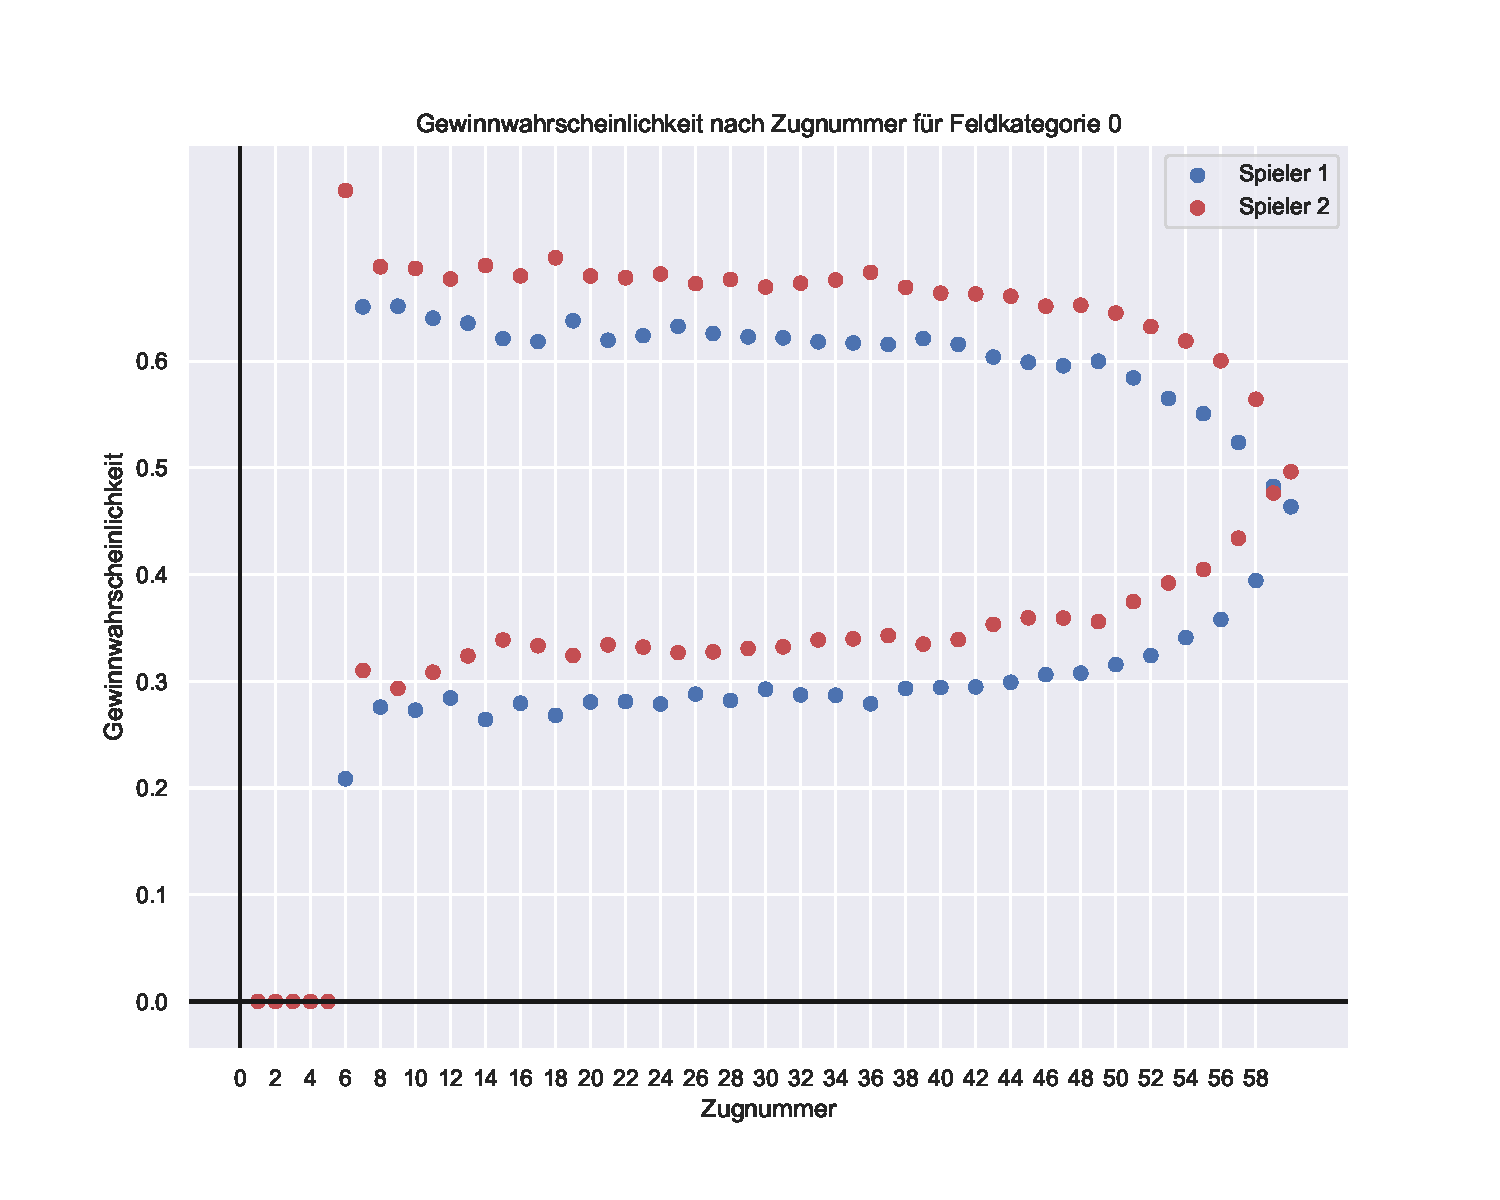
\epsfig{file=Bilder/Field_Cat_Eval/othello-scatter-field_category0.pdf, width=10cm}
\caption{Gewinnwahrscheinlichkeit nach Zug für Feld-Kategorie 0}
\label{fig:win-pro-fc-0}
\end{figure}
\begin{figure}[ht]
\centering
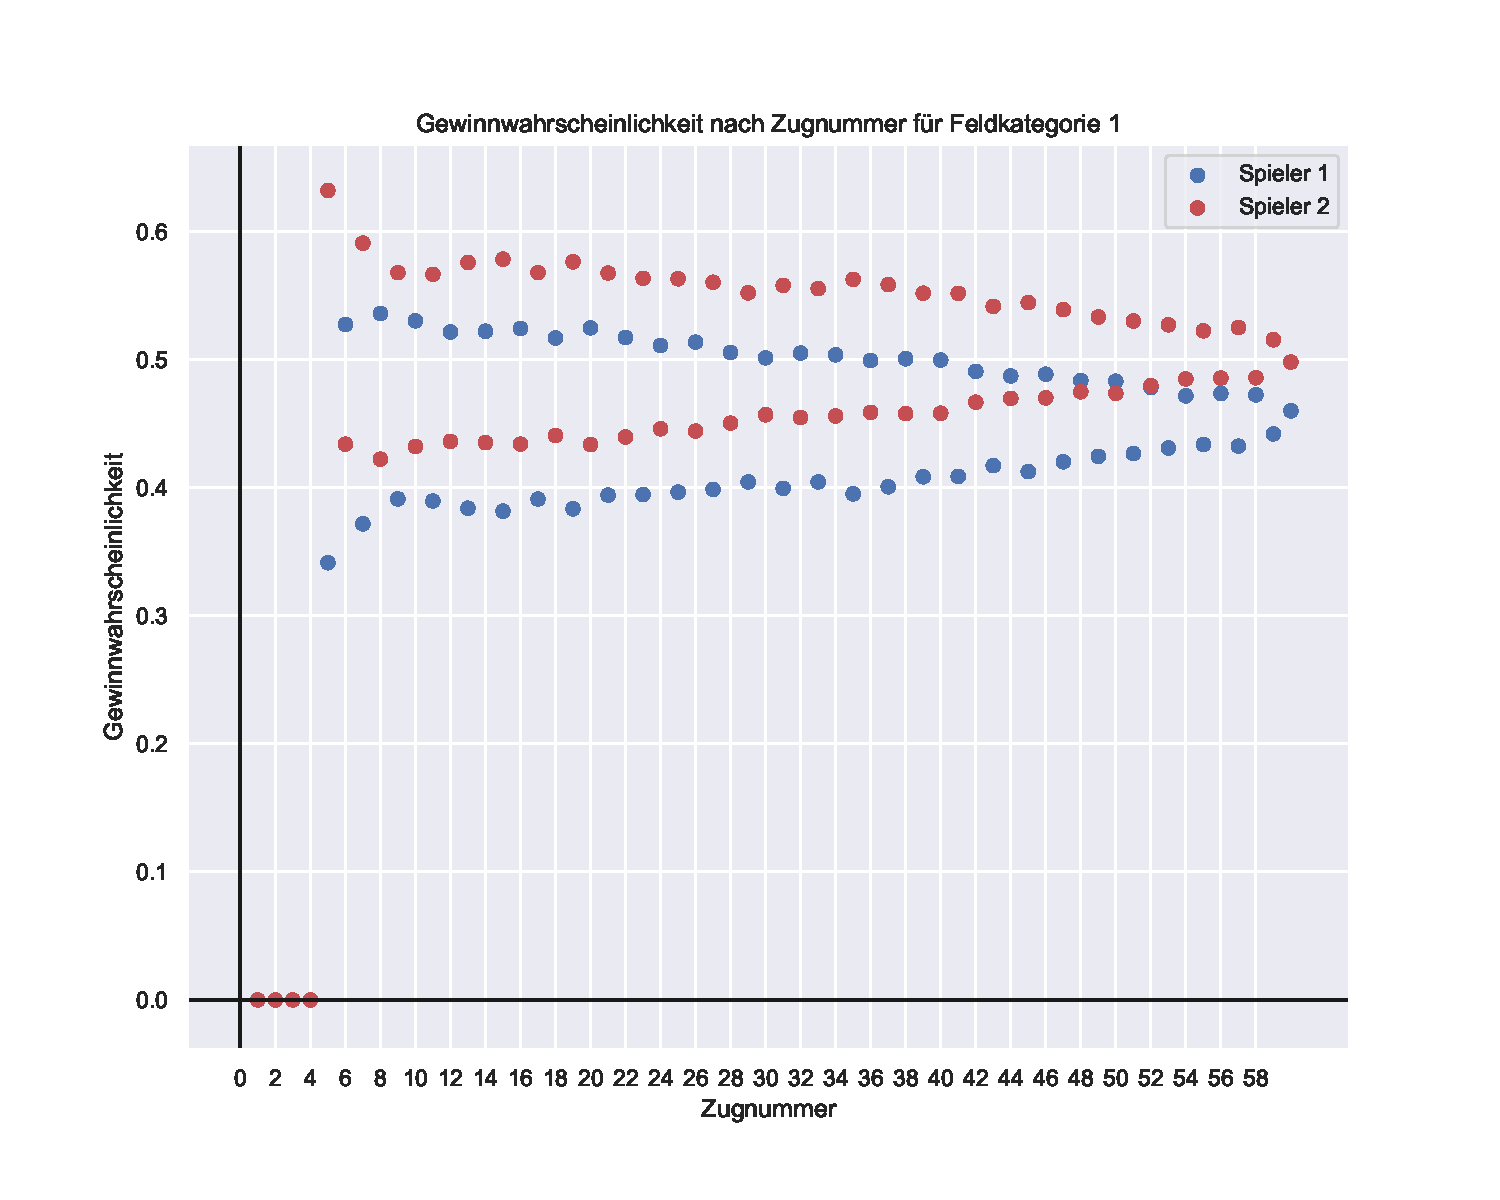
\epsfig{file=Bilder/Field_Cat_Eval/othello-scatter-field_category1.pdf, width=10cm}
\caption{Gewinnwahrscheinlichkeit nach Zug für Feld-Kategorie 1}
\label{fig:win-pro-fc-1}
\end{figure}
\begin{figure}[ht]
\centering
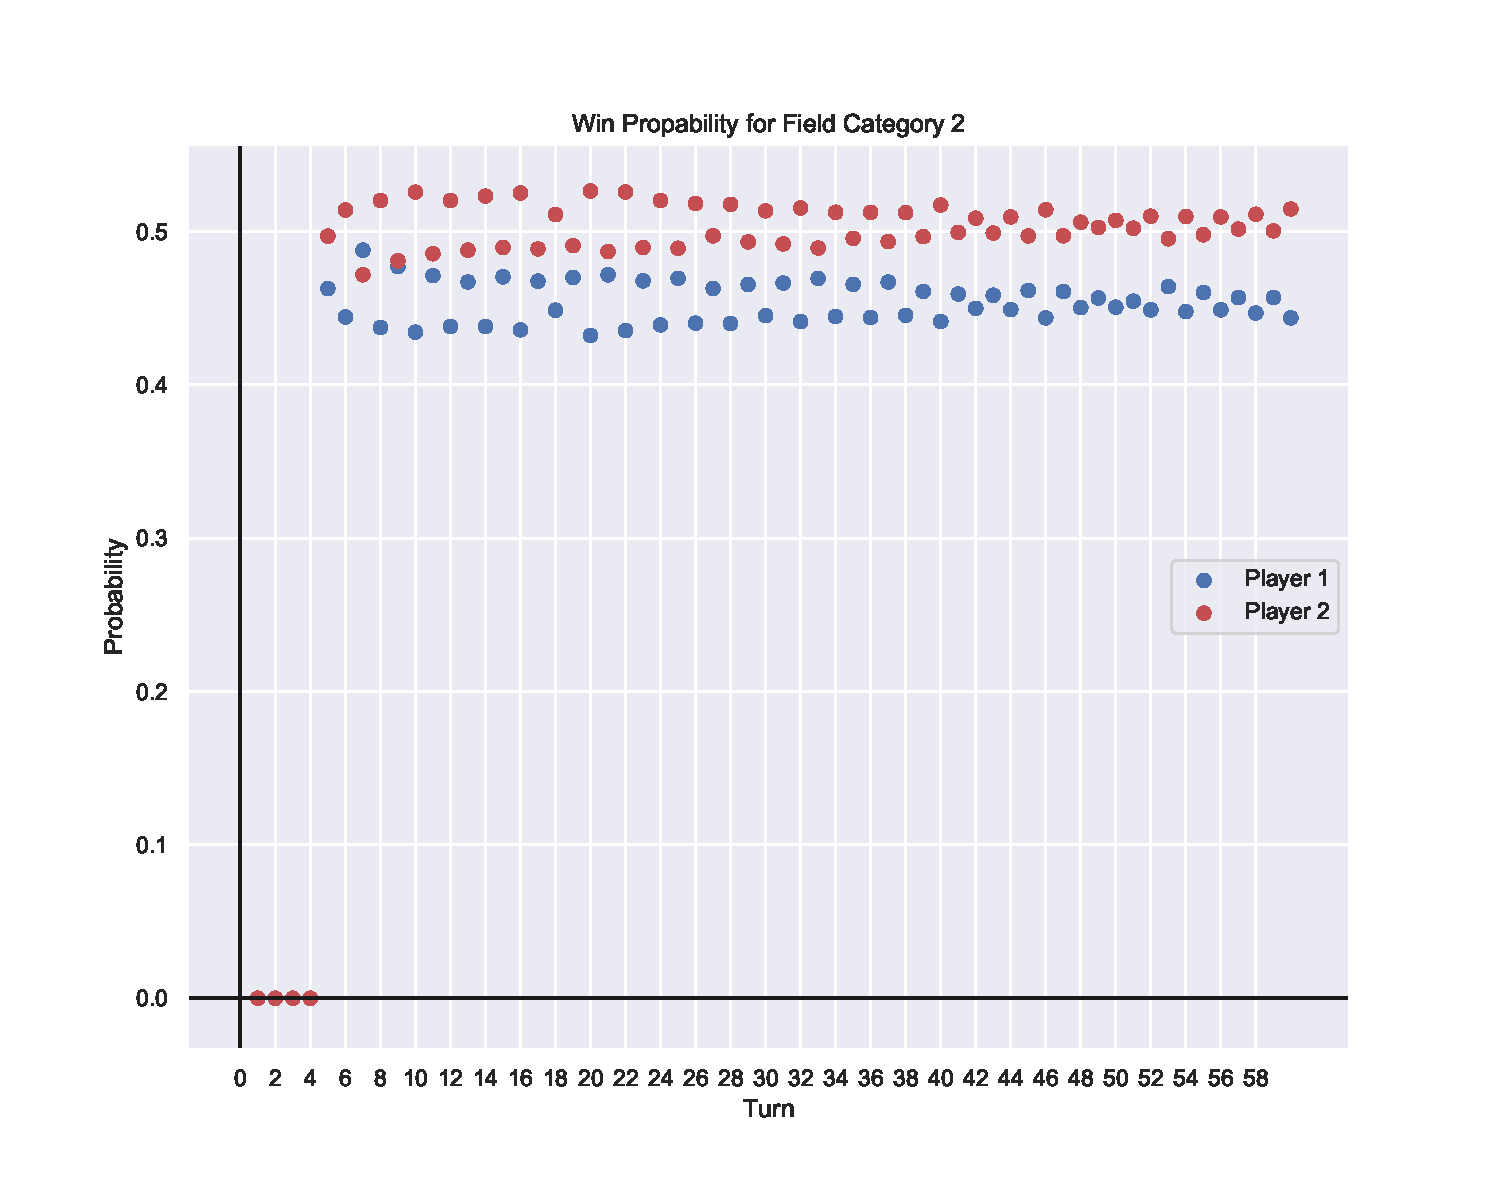
\epsfig{file=Bilder/Field_Cat_Eval/othello-scatter-field_category2.pdf, width=10cm}
\caption{Gewinnwahrscheinlichkeit nach Zug für Feld-Kategorie 2}
\label{fig:win-pro-fc-2}
\end{figure}
\begin{figure}[ht]
\centering
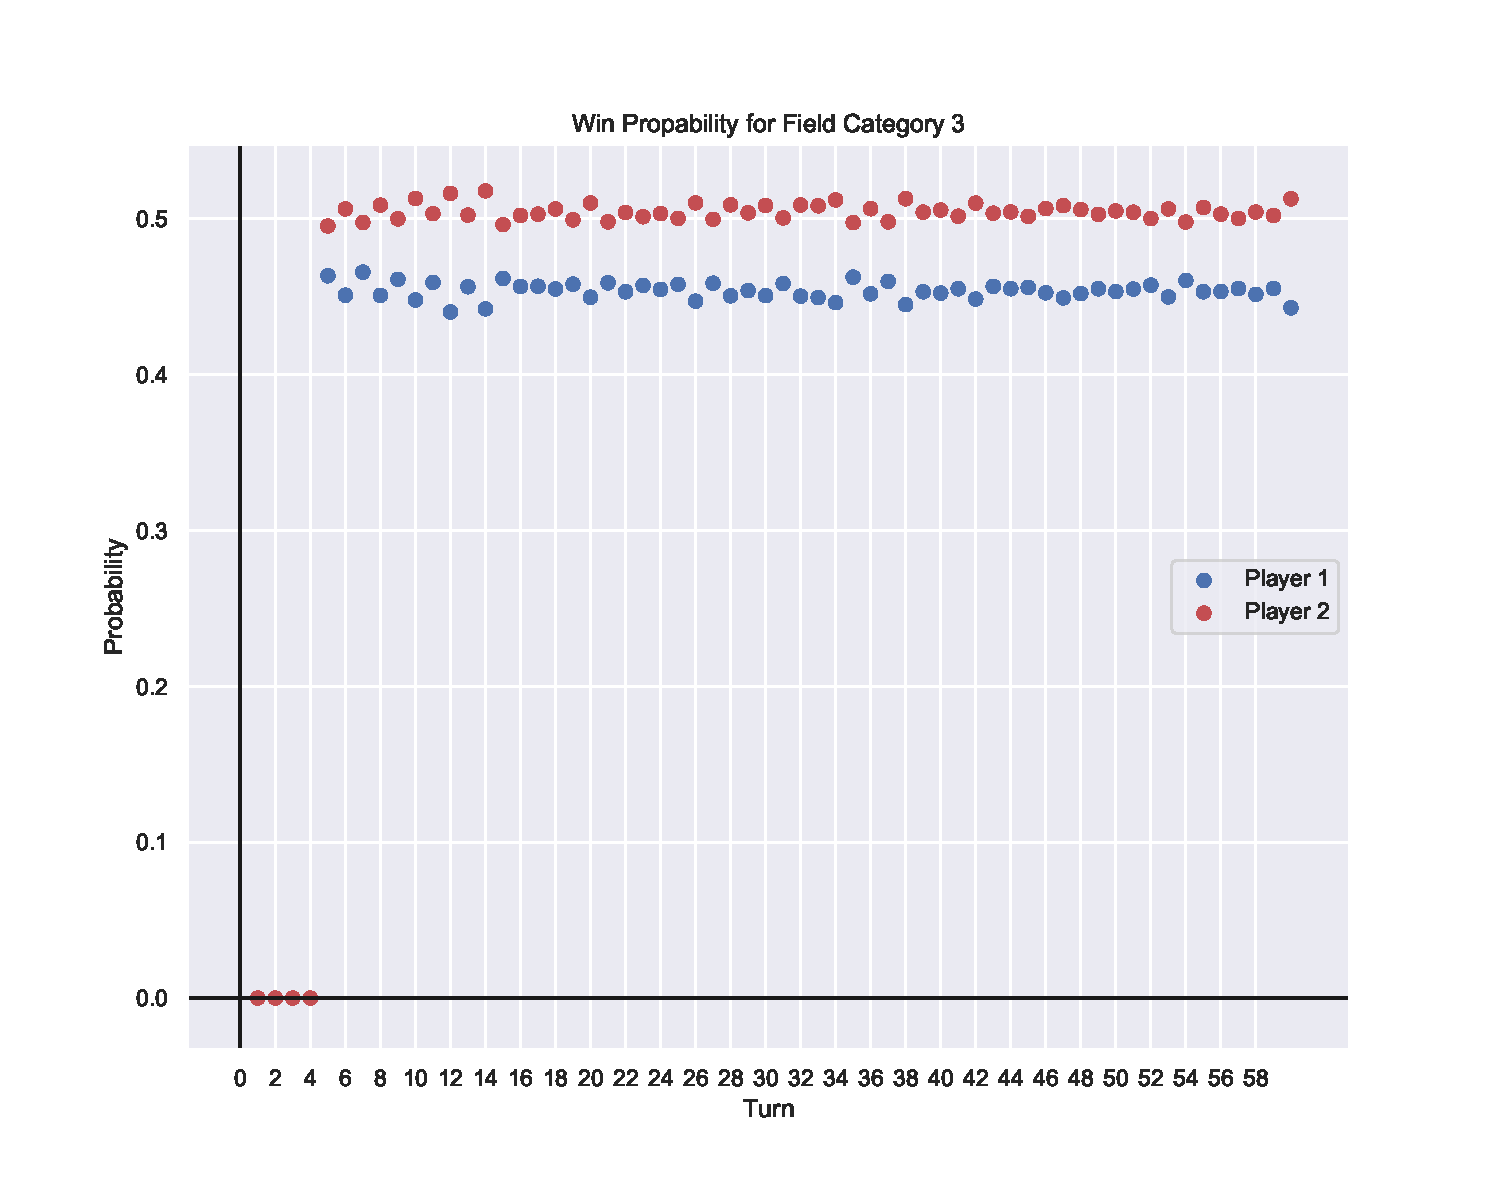
\epsfig{file=Bilder/Field_Cat_Eval/othello-scatter-field_category3.pdf, width=10cm}
\caption{Gewinnwahrscheinlichkeit nach Zug für Feld-Kategorie 3}
\label{fig:win-pro-fc-3}
\end{figure}
\begin{figure}[ht]
\centering
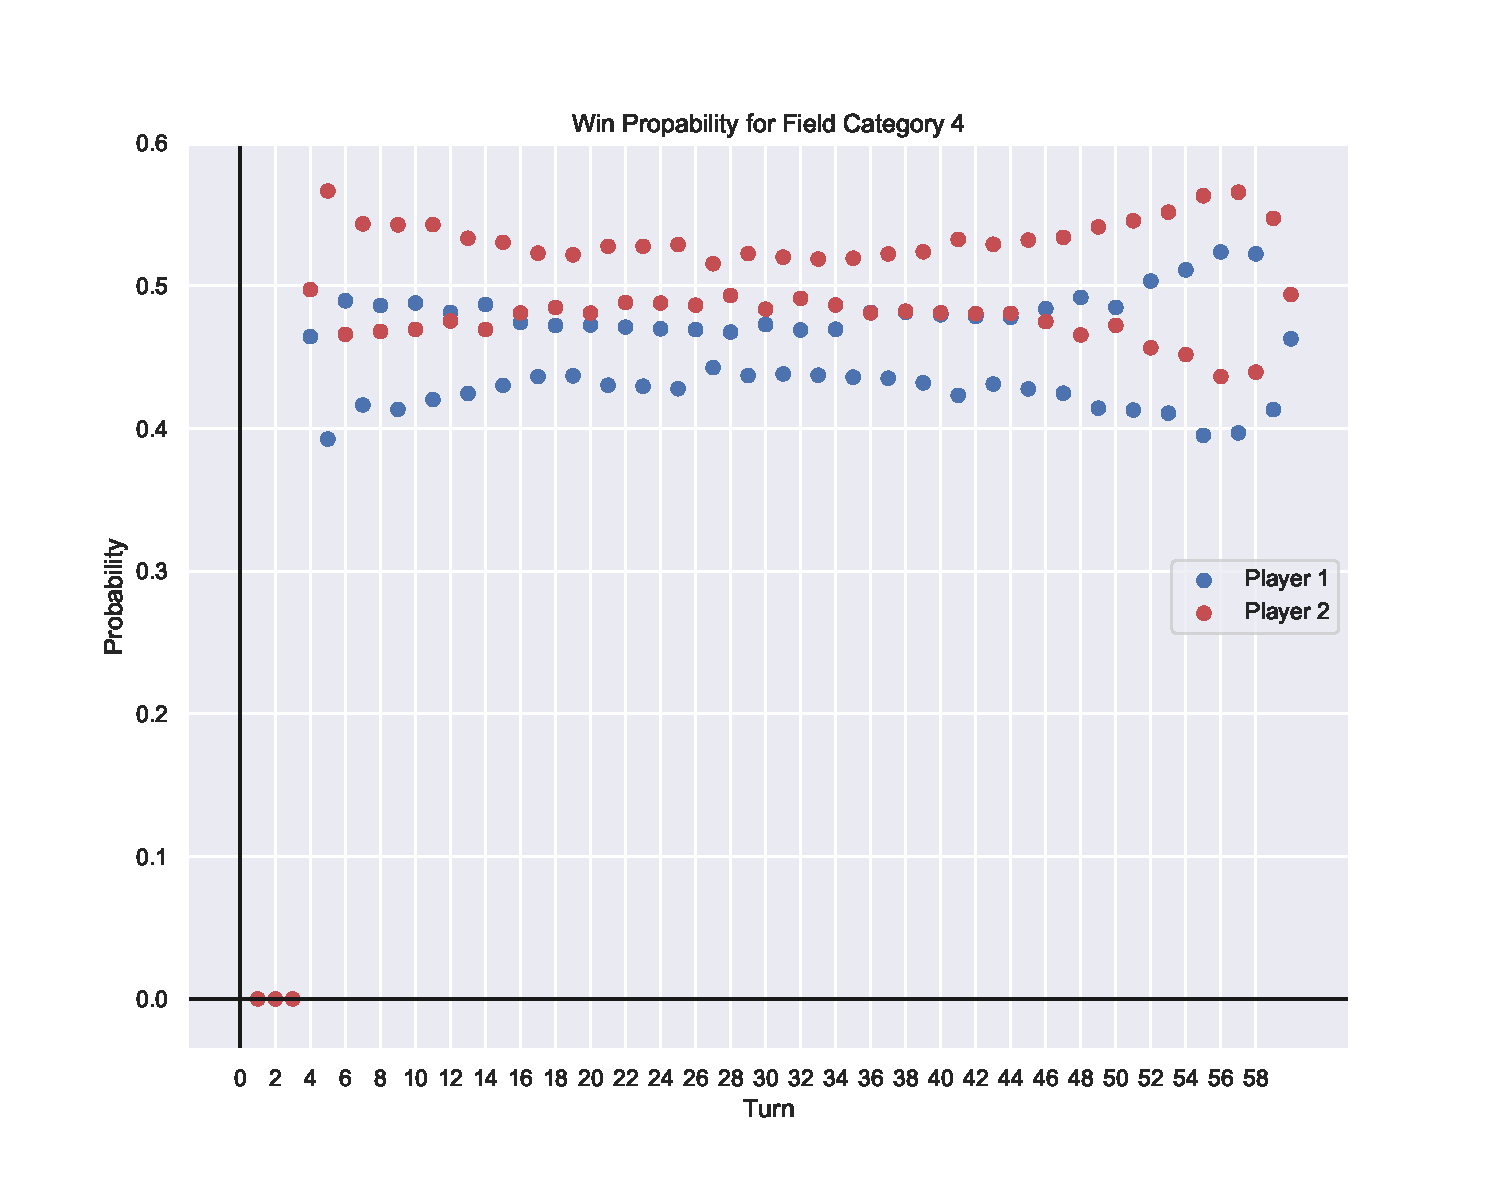
\epsfig{file=Bilder/Field_Cat_Eval/othello-scatter-field_category4.pdf, width=10cm}
\caption{Gewinnwahrscheinlichkeit nach Zug für Feld-Kategorie 4}
\label{fig:win-pro-fc-4}
\end{figure}
\begin{figure}[ht]
\centering
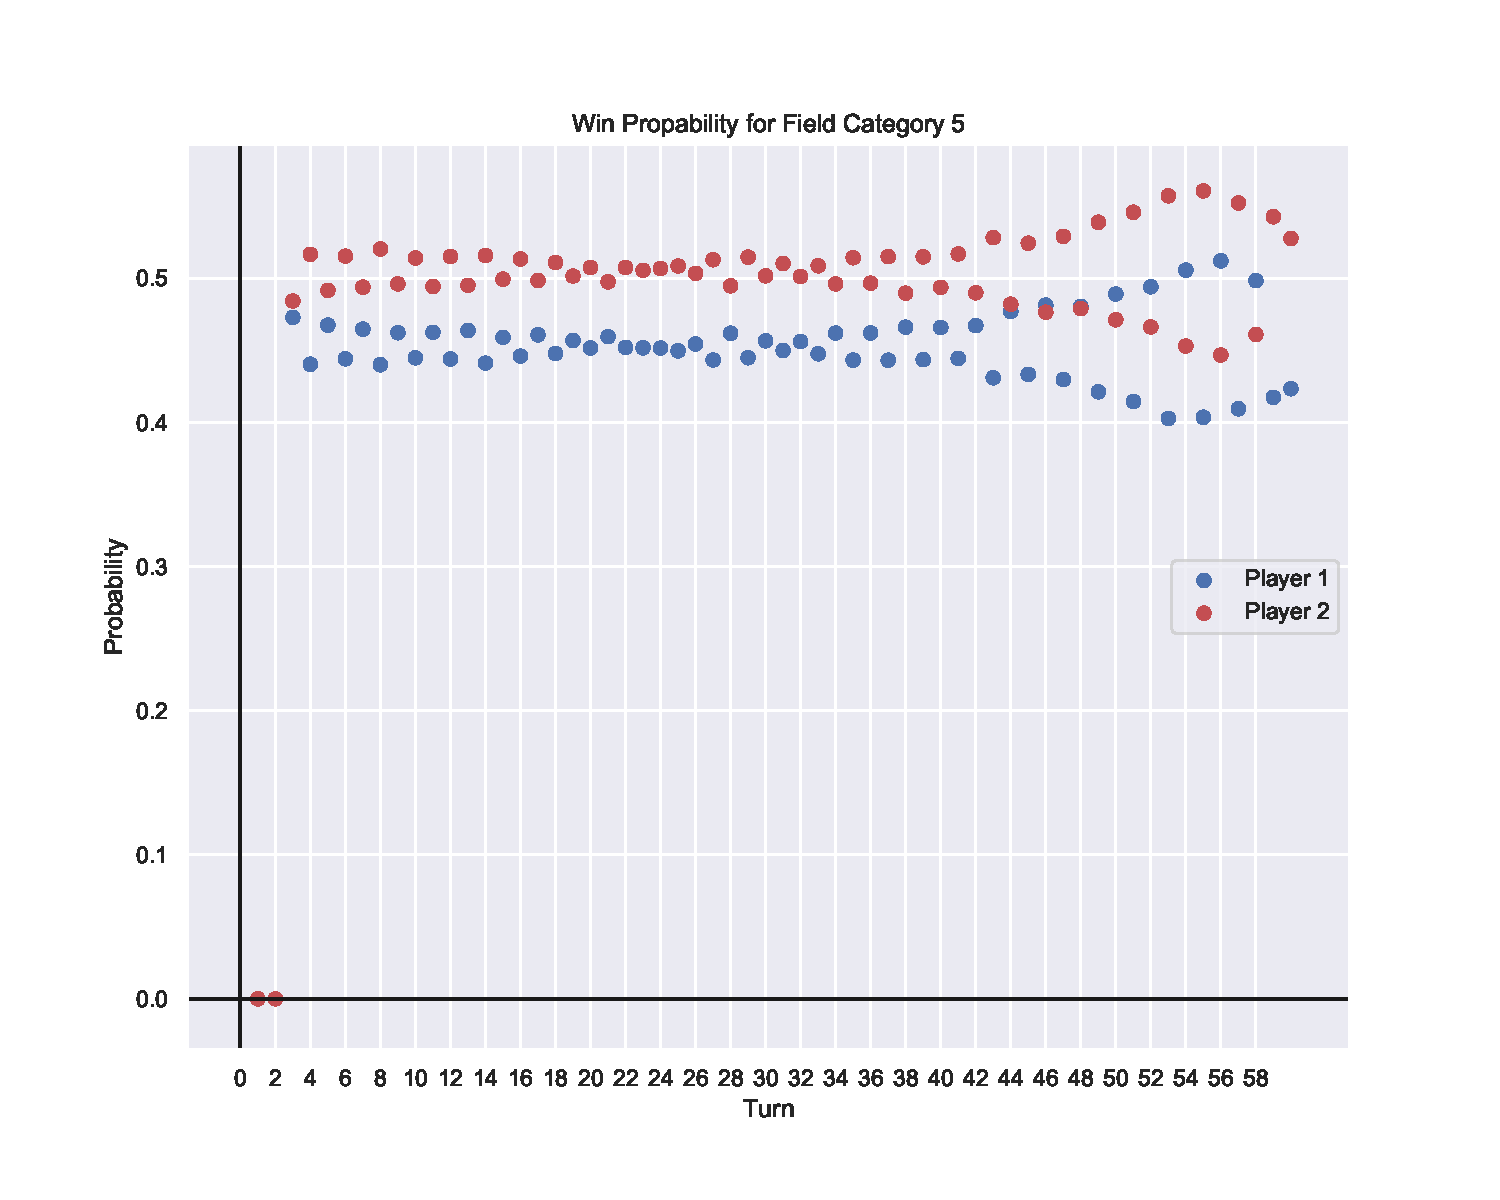
\epsfig{file=Bilder/Field_Cat_Eval/othello-scatter-field_category5.pdf, width=10cm}
\caption{Gewinnwahrscheinlichkeit nach Zug für Feld-Kategorie 5}
\label{fig:win-pro-fc-5}
\end{figure}
\begin{figure}[ht]
\centering
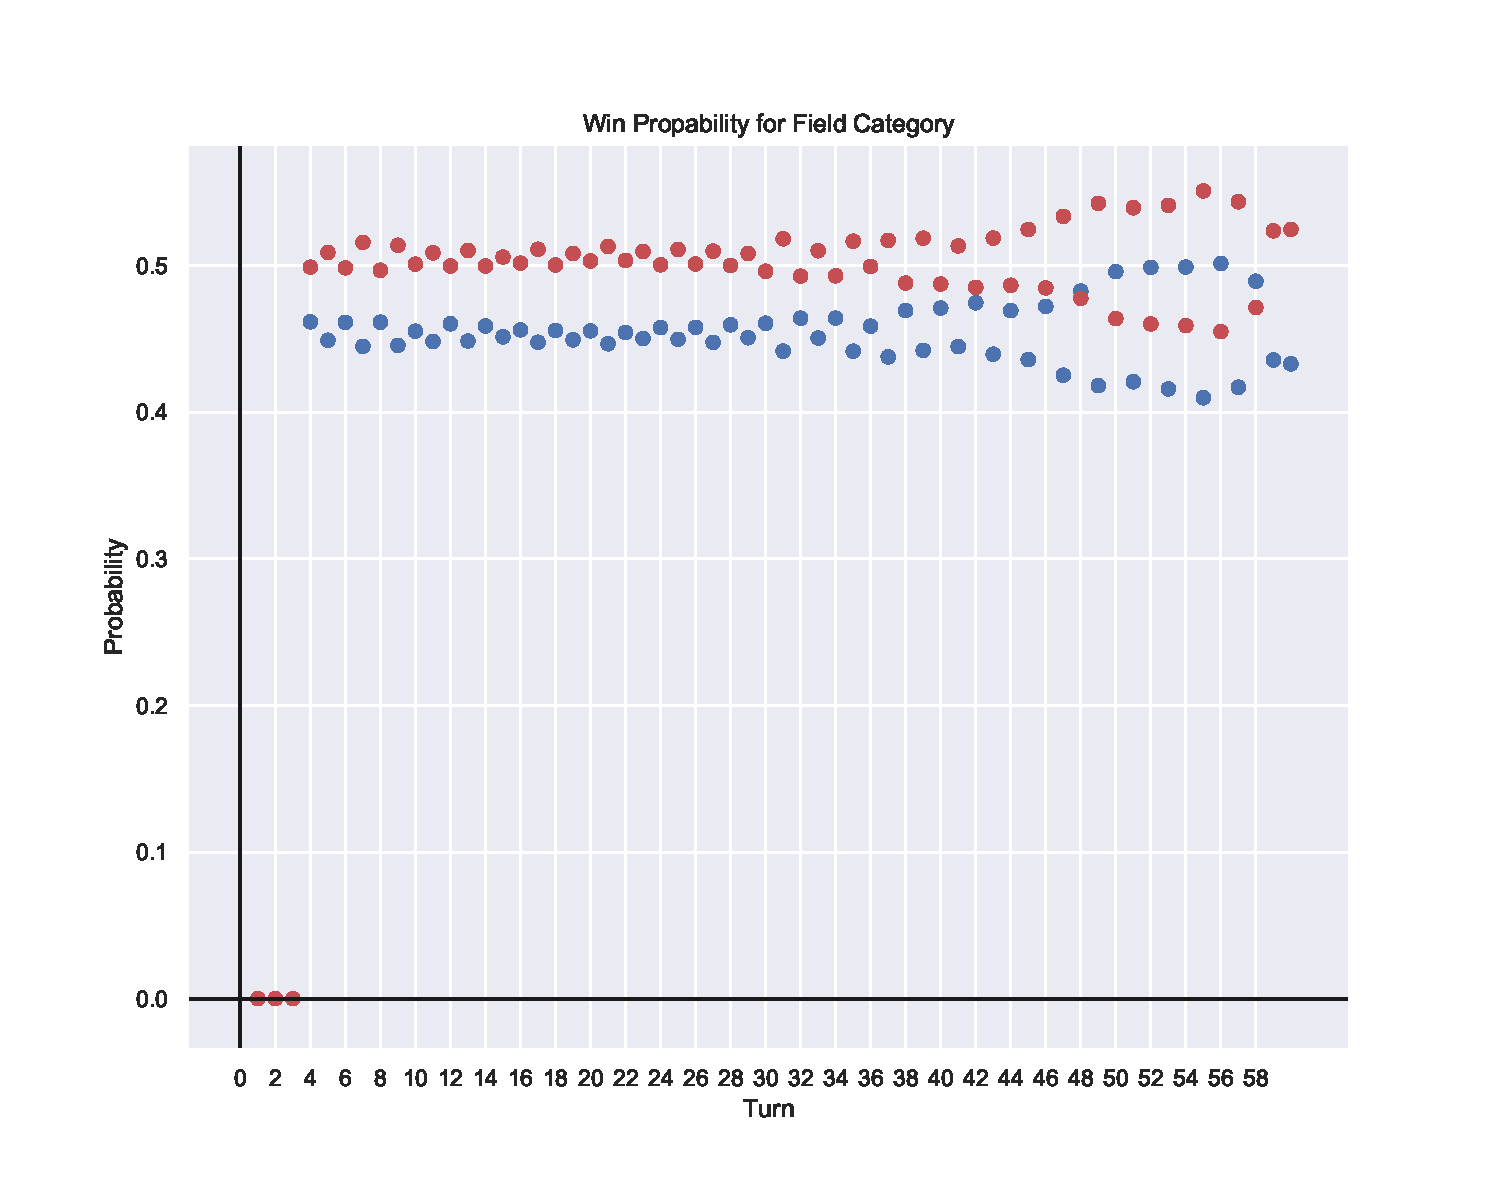
\epsfig{file=Bilder/Field_Cat_Eval/othello-scatter-field_category6.pdf, width=10cm}
\caption{Gewinnwahrscheinlichkeit nach Zug für Feld-Kategorie 6}
\label{fig:win-pro-fc-6}
\end{figure}
\begin{figure}[ht]
\centering
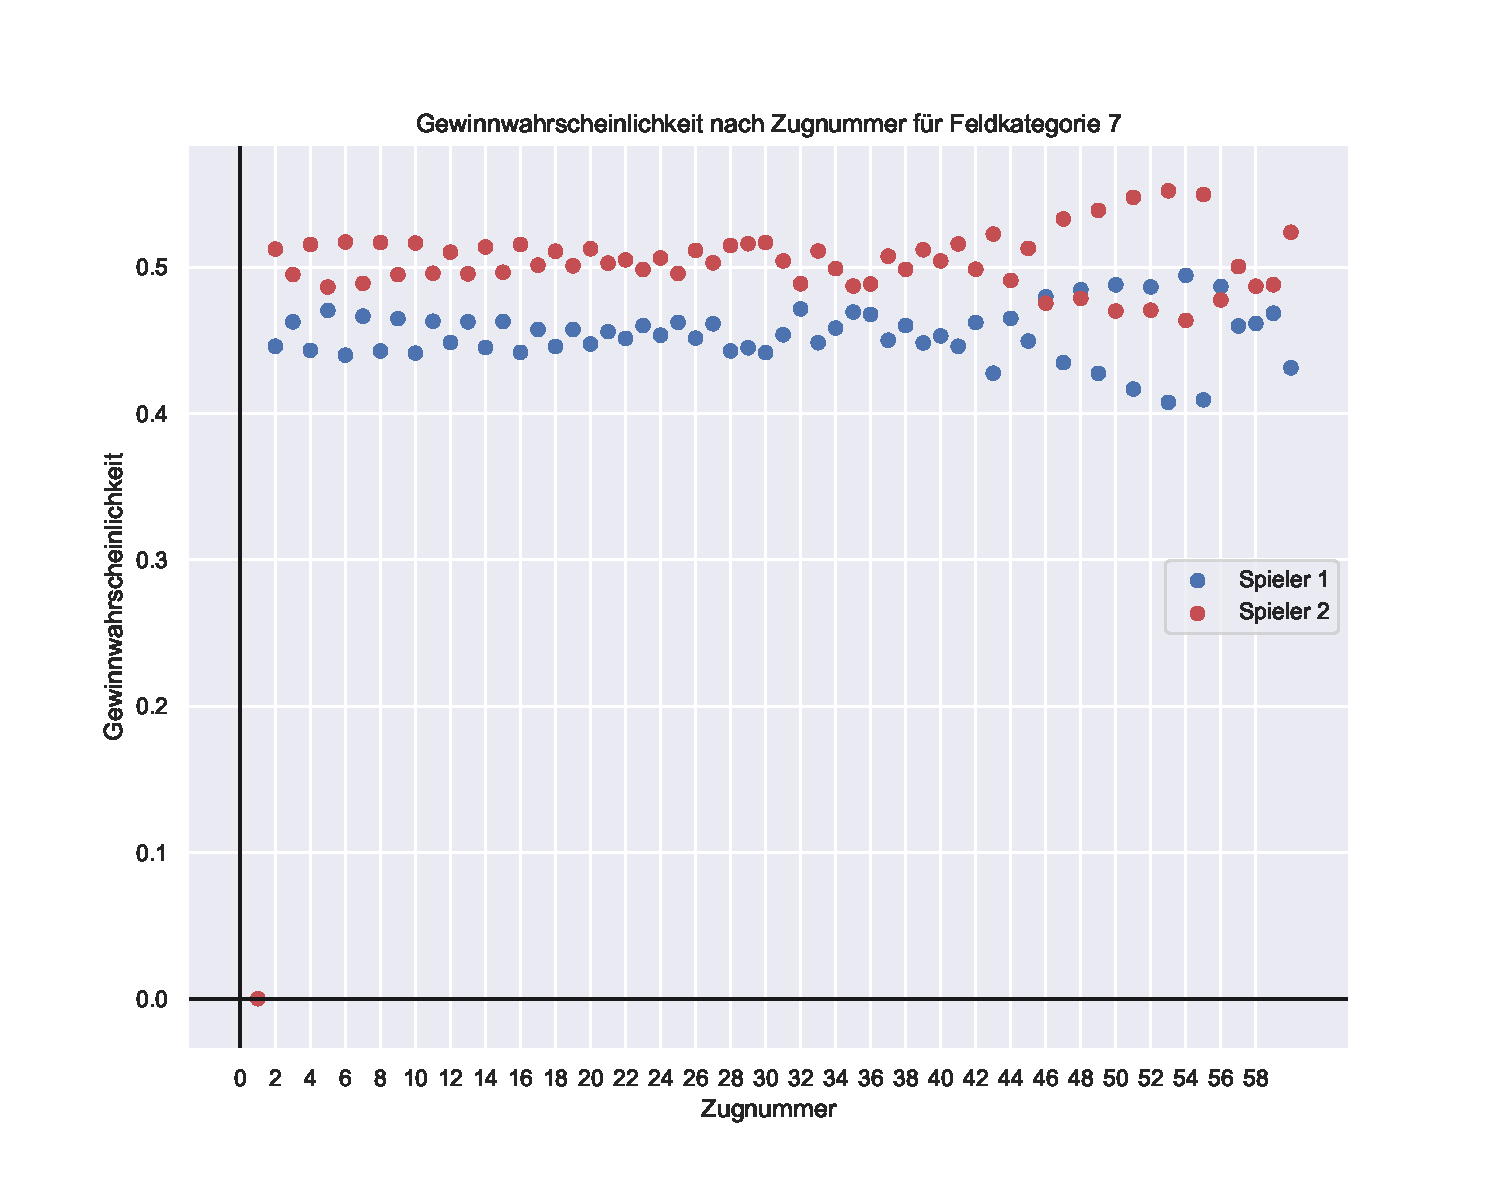
\epsfig{file=Bilder/Field_Cat_Eval/othello-scatter-field_category7.pdf, width=10cm}
\caption{Gewinnwahrscheinlichkeit nach Zug für Feld-Kategorie 7}
\label{fig:win-pro-fc-7}
\end{figure}
\begin{figure}[ht]
\centering
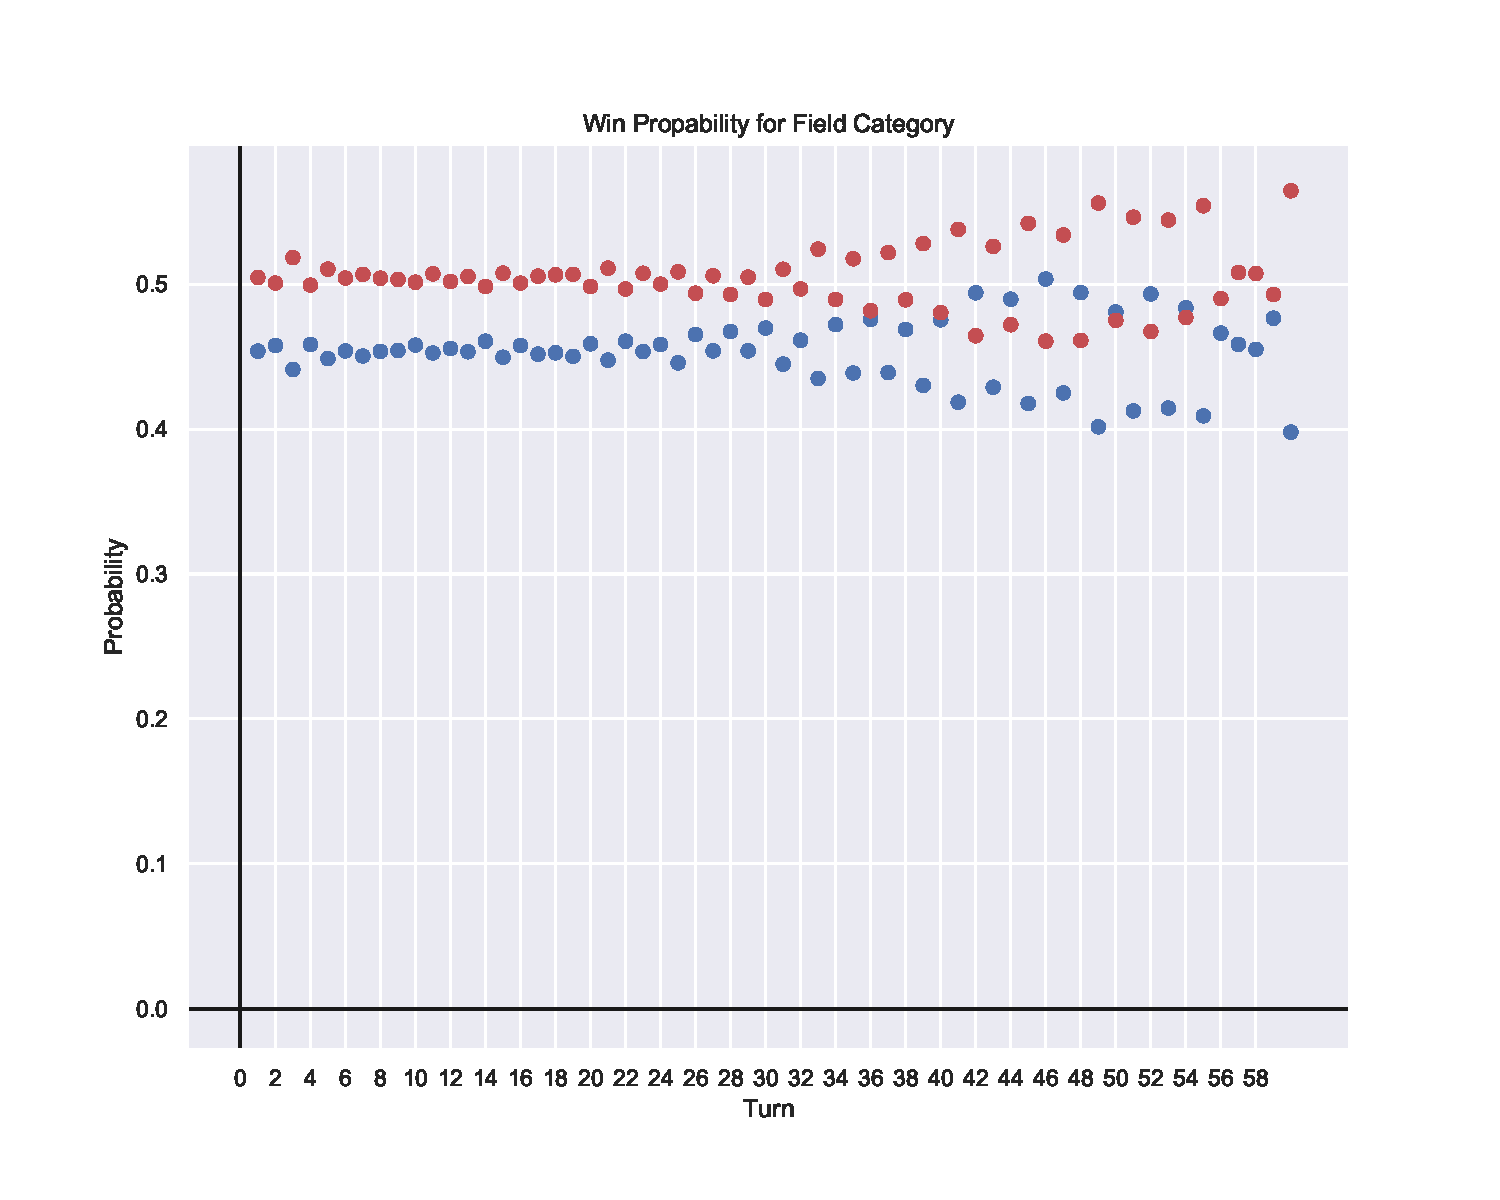
\epsfig{file=Bilder/Field_Cat_Eval/othello-scatter-field_category8.pdf, width=10cm}
\caption{Gewinnwahrscheinlichkeit nach Zug für Feld-Kategorie 8}
\label{fig:win-pro-fc-8}
\end{figure}



\begin{figure}[ht]
\centering
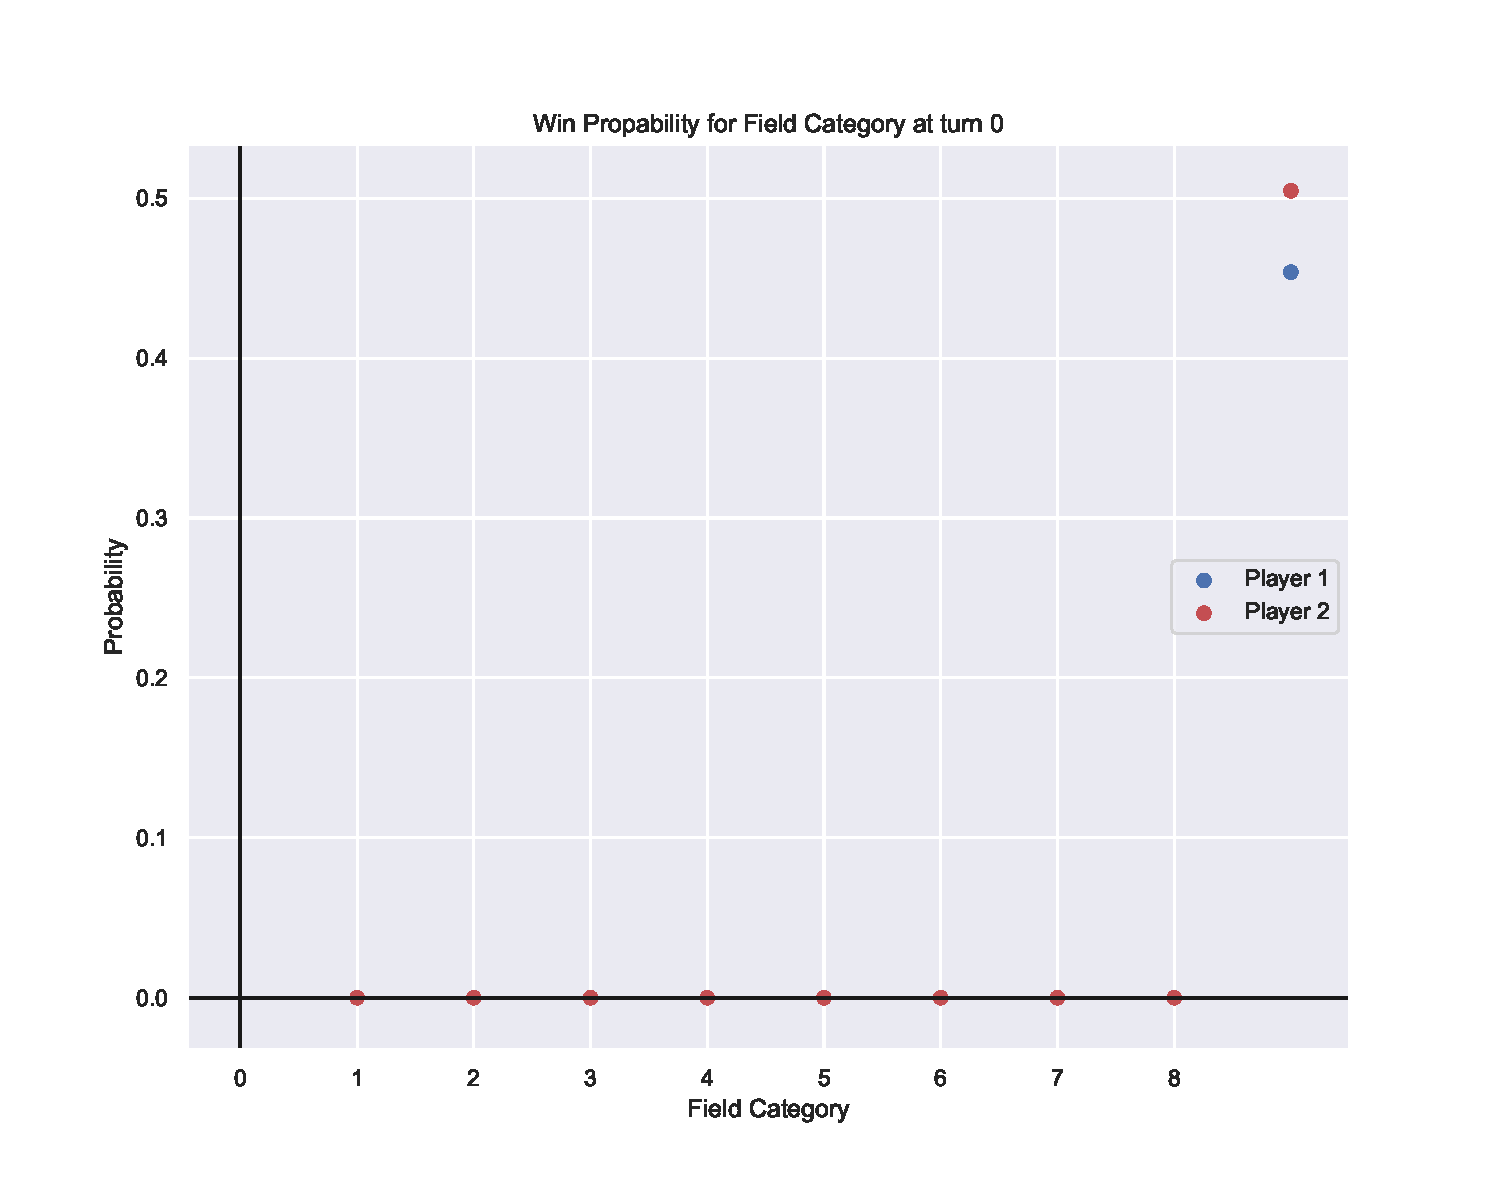
\epsfig{file=Bilder/Field_Cat_Eval/othello-scatter-field_category-by_turn0.pdf, width=10cm}
\caption{Gewinnwahrscheinlichkeit nach Feld Kategorie für Zug Nummer 0}
\label{fig:win-pro-turn-0}
\end{figure}
%Add missing Figures 
\begin{figure}[ht]
\centering
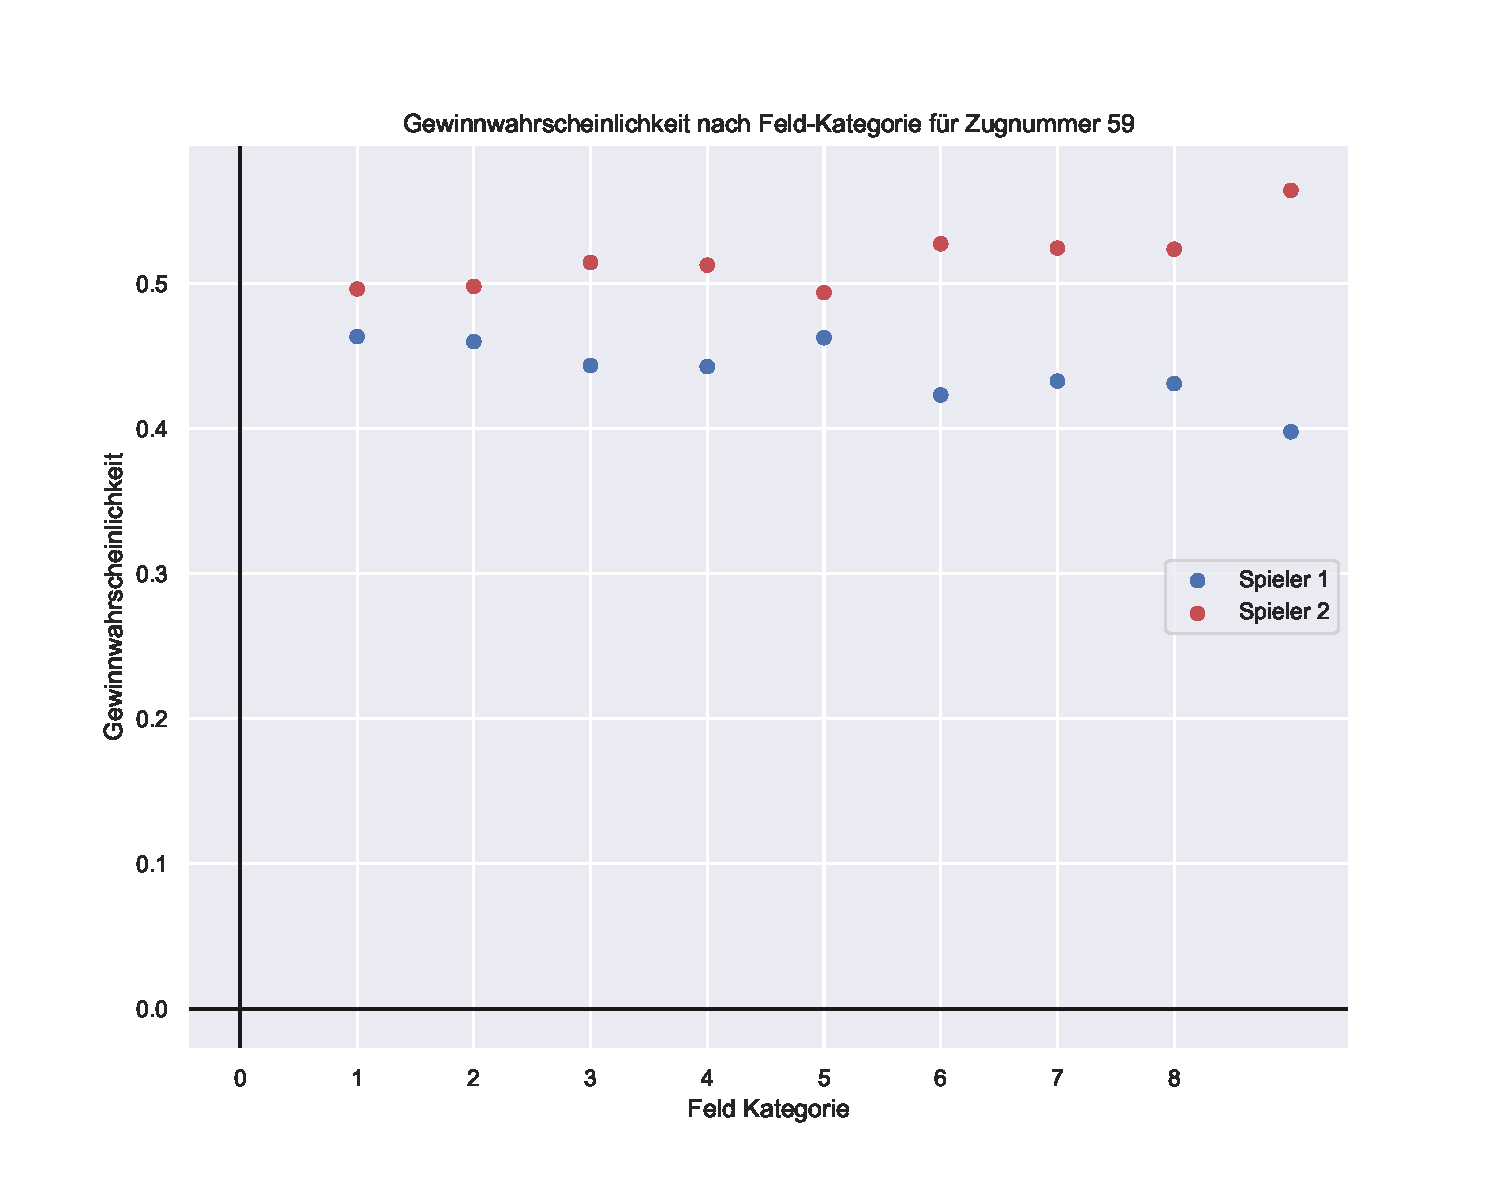
\epsfig{file=Bilder/Field_Cat_Eval/othello-scatter-field_category-by_turn59.pdf, width=10cm}
\caption{Gewinnwahrscheinlichkeit nach Feld Kategorie für Zug Nummer 59}
\label{fig:win-pro-turn-59}
\end{figure}

% später entfernen!! ----------------------------------------
%\newpage
%\listoftodos[Notes]
% -----------------------------------------------------------

% 	Algorithmenverzeichnis
%\listofalgorithms

%	Literaturverzeichnis
\printbibliography[title=Literaturverzeichnis]
\cleardoublepage


%\bibliographystyle{alpha}
%\bibliography{quellen}

\end{document}
